\documentclass[openany]{book}
\usepackage{hyperlatex}
\usepackage{hyperref}
\usepackage{graphicx}

\texonly{\parindent=0in}
\texonly{\oddsidemargin=0in}
\texonly{\evensidemargin=0in}
\texonly{\textwidth=6.0in}
\texonly{\textheight=8.0in}

\htmlonly{\newcommand\code[1]{{\tt #1}}}
\htmlonly{\newcommand\url[1]{\xlink{#1}{#1}}}

\texonly{\renewcommand\code[1]{\path{#1}}}
\texonly{\renewcommand\xlink[2]{\href{#2}{#1}}}
\newcommand\bh{{\bf h}}
\newcommand\bi{{\bf i}}
\newcommand\bo{{\bf o}}
\newcommand\bt{{\bf t}}
\newcommand\bm{{\bf m}}
\newcommand\be{{\bf e}}
\newcommand\bg{{\bf f}}
\newcommand\bb{{\bf b}}
\newcommand\bl{{\bf l}}
\newcommand\bp{{\bf p}}
\newcommand\br{{\bf r}}
\newcommand\bw{{\bf w}}

\setcounter{htmldepth}{2}
\setcounter{htmlautomenu}{3}

\htmltitle{Chord}
\htmladdress{mhn@cs.stanford.edu}

\title{Chord: A Versatile Platform for Program Analysis}
\author{Mayur Naik}
\date{\today}
\begin{document}
\maketitle

\section{What is Chord?}
\label{sec:whatis-chord}

Chord is a program analysis platform that enables 
productively design, implement, evaluate, and combine a
broad variety of program analyses for Java bytecode. It has the
following key features:

\begin{itemize}
\item
{\bf Stand-alone:} It provides various off-the-shelf analyses (e.g., various
call-graph analyses; points-to analyses; thread-escape analysis;
static slicing; static and dynamic concurrency analyses for finding
races, deadlocks, and atomicity violations; etc.)

\item
{\bf Flexible:} It allows users to express a broad range of analyses,
including both static and dynamic analyses, analyses written
imperatively in Java or declaratively in Datalog, summary-based as
well as cloning-based inter-procedural context-sensitive analyses,
iterative refinement-based analyses, client-driven analyses, and
combined static/dynamic analyses.

\item
{\bf Efficient:} It executes analyses in a demand-driven fashion, caches
results computed by each analysis for reuse by other analyses without
re-computation, and can execute analyses without dependencies between
them in parallel.

\item
{\bf Deterministic:} It guarantees that the result is the same regardless of
the order in which different analyses are executed; moreover, results
can be shared across different runs.
\end{itemize}

\noindent Chord is intended to work on a variety of platforms,
including Linux, Windows/Cygwin, and MacOS.  It has been tested most
extensively on Linux.  It is open source software distributed under
the \xlink{New BSD License}{http://www.opensource.org/licenses/bsd-license.php}.
Improvements by users are welcome and encouraged.  The project website
is \url{http://chord.stanford.edu/} and the software development website is
\url{http://jchord.googlecode.com/}.



\xname{getting_started}
\chapter{Getting Started}
\label{chap:getting-started}


This chapter describes how to download, install, and run Chord.
Section \ref{sec:downloading-binaries} describes how to obtain
pre-built binaries of Chord.  Section \ref{sec:downloading-sources}
describes how to obtain the source code of Chord and Section
\ref{sec:downloading-sources} explains how to build it.  Finally,
Section \ref{sec:running-chord} describes how to run Chord.

\section{Downloading Binaries}
\label{sec:downloading-binaries}

To obtain Chord's pre-built binaries, download and uncompress file
\xlink{chord-bin-2.0.tar.gz}{http://jchord.googlecode.com/files/chord-bin-2.0.tar.gz}.
It contains the following files:

\begin{enumerate}
\item
\code{chord.jar}, which contains the class files of Chord and of
libraries used by Chord.
\item
\code{libbuddy.so}, \code{buddy.dll}, and \code{libbuddy.dylib}: you
can keep one of these files depending upon whether you intend to run
Chord on Linux, Windows/Cygwin, or MacOS, respectively.  These files
are needed only if you want BDD library BuDDy to be used when the
BDD-based Datalog solver bddbddb in Chord runs analyses written in
Datalog.
\item
\code{libchord_instr_agent.so}: this file is needed only if you want
the JVMTI-based bytecode instrumentation agent to be used when Chord
runs dynamic analyses.
\end{enumerate}

Novice users can ignore items (2) and (3) until they become more
familiar with Chord.  The binaries mentioned in items (2) and (3)
might not be compatible with your machine, in which case you can
either forgo using them (with hardly any noticeable difference in
functionality), or you can download the sources (see Section
\ref{sec:downloading-sources}) and build them yourself (see Section
\ref{sec:compiling-sources}).

\section{Downloading Source Code}
\label{sec:downloading-sources}

To obtain Chord's source code, download and uncompress the following
files:

\begin{itemize}
\item
Mandatory: file
\xlink{chord-src-2.0.tar.gz}{http://jchord.googlecode.com/files/chord-src-2.0.tar.gz},
which contains Chord's source code and jars of libraries used by
Chord.
\item
Optional: file
\xlink{chord-libsrc-2.0.tar.gz}{http://jchord.googlecode.com/files/chord-libsrc-2.0.tar.gz},
which contains the source code of libraries used by Chord (e.g., joeq,
javassist, bddbddb, etc.)
\end{itemize}

Alternatively, you can obtain the latest development snapshot from the
SVN repository by running the following command:

\begin{verbatim}
    prompt> svn checkout http://jchord.googlecode.com/svn/trunk/ chord
\end{verbatim}

Instead of checking out the entire \code{trunk/}, which contains
several sub-directories, you can check out specific sub-directories:

\begin{itemize}
\item
\code{main/} contains Chord's source code and jars of libraries used by Chord.
\item
\code{libsrc/} contains the source code of libraries used by Chord
(e.g., joeq, javassist, bddbddb, etc.).
\item
\code{test/} contains Chord's regression tests.
\item
many more; these might eventually move into \code{main/}.
\end{itemize}

Files \code{chord-2.0-src.tar.gz} and \code{chord-2.0-libsrc.tar.gz}
mentioned above are essentially stable releases of the \code{main/}
and \code{libsrc/} directories, respectively.

\section{Compiling the Source Code}
\label{sec:compiling-sources}

Compiling Chord's source code requires the following software:

\begin{itemize}
\item
A JVM with JDK 5 or higher, e.g.
\xlink{IBM J9}{http://www.ibm.com/developerworks/java/jdk/} or
\xlink{Oracle HotSpot}{http://www.oracle.com/technetwork/java/javase/downloads/index.html}.
\item
\xlink{Apache Ant}{http://ant.apache.org/}, a Java build tool.
\end{itemize}

Chord's main directory contains a file named {\tt build.xml} which is
interpreted by Apache Ant.  To see the various possible targets,
simply run command ``{\tt ant}" in that directory.

To compile Chord, run command ``{\tt ant compile}" in the same directory.
This will compile Chord's Java sources from \code{src/} to class
files in \code{classes/}, as well as build a jar file
\code{chord.jar} that contains these class files as well as those
in the jars of libraries that are used by Chord and are
provided under \code{lib/} (e.g., \code{joeq.jar},
\code{javassist.jar}, \code{bddbddb.jar}, etc.).  Additionally:

\begin{itemize}
\item

If system property \code{chord.use.buddy} is set to \code{true}, then
the C source code of BDD library
\xlink{BuDDy}{http://buddy.sourceforge.net/} from directory \code{bdd/}
will be compiled to a shared library named
(\code{libbuddy.so} on Linux, \code{buddy.dll} on Windows, and
\code{libbuddy.dylib} on MacOS; this library is used by BDD-based
Datalog solver \xlink{bddbddb}{http://bddbddb.sourceforge.net/} in
Chord for running analyses written in Datalog.

\item

If system property \code{chord.use.jvmti} is set to \code{true}, then
the C++ source code of the JVMTI-based bytecode instrumentation agent
from directory \code{agent/} will be compiled to a shared library named
\code{libchord_instr_agent.so} on all architectures;
this agent is used in Chord for computing analysis scope dynamically
and for running dynamic analyses.
\end{itemize}

Properties \code{chord.use.buddy} and \code{chord.use.jvmti} are
defined in file \code{chord.properties} in Chord's main directory.
The default value of both these properties is \code{false}.  If you set
either of them to \code{true}, then you will also need a utility like
GNU Make (to run the \code{Makefile}'s in directories \code{bdd/} and
\code{agent/}) and a C++ compiler.

\section{Running Chord}
\label{sec:running-chord}

Running Chord requires a JVM with JDK 5 or higher.
There are two equivalent ways to run Chord.
One way, which is available only in the source installation of Chord, is to run the
following command in Chord's main directory:

\begin{verbatim}
    prompt> ant -D<key1>=<value1> ... -D<keyN>=<valueN> run
\end{verbatim}

The above requires Apache Ant (a Java build tool) to be installed on
your machine.  The alternative, which does not require Apache Ant and is
available in both the source and binary installations of Chord, is
to run the following command:

\begin{verbatim}
    prompt> java -cp <...>/chord.jar -D<key1>=<value1> ... -D<keyN>=<valueN> chord.project.Boot
\end{verbatim}

where \code{<...>} denotes the absolute or relative path of the
directory containing file \code{chord.jar}; that directory is also
expected to contain any other binaries in Chord's installation (e.g.,
\code{libbuddy.so} and \code{libchord_instr_agent.so}).

Each ``\code{-D<key>=<value>}" argument above sets the system property
named \code{<key>} to the value denoted by \code{<value>}.  The only
way to specify inputs to Chord is via system properties; there is no
command-line argument processing.  Chapter\ref{chap:properties}
describes all system properties recognized by Chord.


\xname{example}
\chapter{An Example Run}
\label{chap:example}

This chapter describes how to setup a Java program and run predefined analyses
in Chord on it.

Suppose the Java program to be analyzed has the following directory structure:

\begin{framed}
\begin{verbatim}
example/
    src/
        foo/
            Main.java
            ...
    classes/
        foo/
            Main.class
            ...
    lib/
        src/
            taz/
                ...
        jar/
            taz.jar
    chord.properties
\end{verbatim}
\end{framed}

The above structure is typical: the program's Java source
files are under {\tt src/}, its class files are under {\tt classes/},
the source and jar files of the libraries used by the program are
under \code{lib/src/} and \code{lib/jar/}, respectively.

To run Chord on the above program, run the following command in
Chord's main directory:

\begin{framed}
\begin{verbatim}
ant -Dchord.work.dir=<...>/example run
\end{verbatim}
\end{framed}

where \code{<...>} denotes the absolute or relative path of the
directory containing the above \code{example/} directory.
Property \code{chord.work.dir} specifies the working directory during Chord's execution.
Chord searches for a file named \code{chord.properties} under that directory, and
loads upfront all properties defined in that file, if it exists.  Alternatively, these properties
may be defined on the command-line, using the \code{-D<key>=<value>} format.
A sample \code{chord.properties} file for the above program is as follows:

\begin{framed}
\begin{verbatim}
chord.main.class=foo.Main
chord.class.path=classes:lib/jar/taz.jar
chord.src.path=src:lib/src
chord.run.ids=0,1
chord.args.0="-thread 1 -n 10"
chord.args.1="-thread 2 -n 50"
\end{verbatim}
\end{framed}

Each relative file/directory name in the value of any property
defined in this file (e.g., the \code{lib/src} directory name in the value of
property \code{chord.src.path} above) is treated relative to Chord's working directory
(which is specified by property \code{chord.work.dir}).

Chapter \ref{chap:properties} presents an exhaustive listing of
properties recognized by Chord.  Here, we only describe those defined
in the above sample \code{chord.properties} file:

\begin{itemize}
\item
\code{chord.main.class} specifies the fully-qualified name of the main
class of the program.
\item
\code{chord.class.path} specifies the application classpath
of the program (the standard library classpath is implicitly
included).
\item
\code{chord.src.path} specifies the Java source path of the program.
All program analyses in Chord operate on Java bytecode.  The only use
of this property is to HTMLize the Java source files of the program so
that the results of program analyses can be reported at the Java
source code level.
\item
\code{chord.run.ids} specifies a list of IDs to identify runs of the
program.  It is used by dynamic program analyses to determine how many
times the program must be run.  An additional use of this property is
to allow specifying the command-line arguments to use in the run
having ID {\tt <id>} via property \code{chord.args.<id>}, as
illustrated by properties \code{chord.args.0} and \code{chord.args.1}
in the above example.
\end{itemize}

In the above case, Chord does not do much beyond loading the above
\code{chord.properties} file.  For Chord to do something interesting,
additional properties must be set that specify the task(s)
Chord must perform.  All tasks are summarized in Section \ref{sec:func-props}.
The most common task is to run one or more analyses on an input Java program.
Chord implements many standard analyses, including various may-alias and
call-graph analyses, thread-escape analysis, various concurrency analyses,
etc. Many of these analyses are described in Chapter \ref{chap:predefined-analyses}.
Moreover, users can extend these analyses or define their own ones, as
explained in Chapter \ref{chap:analyses}.
Broadly, there are two kinds of analyses in Chord:

\begin{itemize}
\item
Those expressed imperatively in Java. They are in \code{*.java} files under
directory \code{main/src/chord/analyses/}, and are of the form:

\begin{framed}
\begin{verbatim}
@Chord(
    name=<JAVA ANALYSIS NAME>
    ...
)
public class XYZ extends ... {
    ...
}
\end{verbatim}
\end{framed}

\item

Those expressed declaratively in Datalog.  They are in \code{*.dlog} files under
directory \code{main/src/chord/analyses/}, and are of the form:

\begin{framed}
\begin{verbatim}
# name=<DLOG ANALYSIS NAME>

# Program domains
.include ...
.include ...

# BDD variable order
.bddvarorder ...
\end{verbatim}
\end{framed}
\end{itemize}

To run one or more such analyses, run the following command in Chord's main directory:

\begin{framed}
\begin{verbatim}
ant -Dchord.work.dir=<PROGRAM DIR> -Dchord.run.analyses=<ANALYSIS NAME> run
\end{verbatim}
\end{framed}

where {\tt <PROGRAM DIR>} denotes a directory containing a Java program as described above,
and {\tt <ANALYSIS NAME>} denotes the name of an analysis to run,
such as {\tt <JAVA ANALYSIS NAME>} and {\tt <DLOG ANALYSIS NAME>} in the Java and
Datalog analyses depicted above.

For instance, to run a basic may-alias and call-graph analysis (called 0CFA),
run the following command in Chord's main directory:

\begin{framed}
\begin{verbatim}
ant -Dchord.work.dir=<PROGRAM DIR> -Dchord.run.analyses=cipa-0cfa-dlog run
\end{verbatim}
\end{framed}

This instructs Chord to run the Datalog analysis named \code{cipa-0cfa-dlog},
which happens to be defined in file \code{main/src/chord/analyses/alias/cipa_0cfa.dlog}.

The output of the above command is of the form:

\begin{framed}
{\small
\begin{verbatim}
Buildfile: build.xml

run:
     [java] Chord run initiated at: Mar 13, 2011 10:31:08 PM
     [java] ENTER: cipa-0cfa-dlog
     [java] ENTER: T
     [java] ENTER: RTA
     [java] Iteration: 0
     [java] Iteration: 1
     [java] Iteration: 2
     [java] LEAVE: RTA
     [java] SAVING dom T size: 1386
     [java] LEAVE: T
     [java] ENTER: F
     [java] SAVING dom F size: 4120
     [java] LEAVE: F
     ...
     [java] ENTER: MputStatFldInst
     [java] SAVING rel MputStatFldInst size: 739
     [java] LEAVE: MputStatFldInst
     [java] ENTER: statIM
     [java] SAVING rel statIM size: 3359
     [java] LEAVE: statIM
     [java] Starting command: 'java ... chord_analyses_alias_cipa_0cfa.dlog'
     [java] Relation VH: 541 nodes, 449.0 elements (V0,H0)
     [java] Relation FH: 137 nodes, 8.0 elements (H0,F0)
     [java] Relation HFH: 199 nodes, 35.0 elements (H0,F0,H1)
     [java] Relation IM: 590 nodes, 69.0 elements (I0,M0)
     [java] Finished command: 'java ... chord_analyses_alias_cipa_0cfa.dlog'
     [java] LEAVE: cipa-0cfa-dlog
     [java] Chord run completed at: Mar 13, 2011 10:31:36 PM
     [java] Total time: 00:00:27:671 hh:mm:ss:ms

BUILD SUCCESSFUL
Total time: 28 seconds
\end{verbatim}
}
\end{framed}

Notice that although Chord is only asked to run the 0CFA analysis on the command line, it automatically
runs many other analyses before finally running the desired analysis and terminating.
Each analysis in Chord is written modularly, independent of other analyses, along with lightweight
annotations specifying the inputs and outputs of the analysis.  Chord's runtime automatically computes
producer-consumer relationships between analyses (e.g., determines which analysis produces as output a
result that is needed as input by another analysis).  Before running a desired analysis
(such as 0CFA in the above example), Chord recursively runs other analyses until the
inputs to the desired analysis have been computed; it finally runs the desired analysis to produce
the outputs of that analysis.

In the above example, the 0CFA analysis consumes {\it program relations} 
such as \code{MputStatFldInst} and \code{statIM}, each of which is produced by a separate Java analysis with the
corresponding name, and produces program relations \code{VH}, \code{FH}, \code{HFH}, and \code{IM}.

The program relations consumed by the 0CFA analysis contain basic program facts.  For instance,
\code{MputStatFldInst} is a relation containing each tuple ($m$,$f$,$v$) such that method $m$ in the input Java
program contains a putstatic instruction of the form ``$f$ = $v$", while \code{statIM} is a relation
containing each tuple ($i$,$m$) such that $m$ is the target method of invokestatic instruction $i$.

The program relations produced by the 0CFA analysis represent points-to information and the
call graph of the input Java program as computed by the analysis.
Specifically, relations \code{VH}, \code{FH}, and \code{HFH} represent points-to information 
for local variables, static fields, and instance fields, respectively,
while relation \code{IM} represents the call graph, namely, it contain each tuple ($i$,$m$) such that
$m$ is a possible target method of call site $i$.

Metavariables $m$, $f$, $i$, and $v$ above range over entities in so-called {\it program domains} \code{M},
\code{F}, \code{I}, and \code{V}, respectively.
A program domain is a set of entities of a certain kind in the input Java program.  For instance,
\code{M} is the domain representing
the set of all methods in the input Java program, \code{F} is the domain representing the set of all fields,
\code{I} is the domain representing
the set of all call sites in methods in \code{M}, and \code{V} is the domain representing the set of all local variables of reference type in methods in \code{M}.
Each of these domains is produced by a separate Java analysis with the corresponding name.
Notice that the analyses producing these domains run upfront because these domains
are consumed by the analyses that produce relations such as \code{MputStatFldInst} and
\code{statIM}, which in turn are consumed by the desired 0CFA analysis.

During execution, Chord dumps intermediate and final results to files in the
directory specified by property \code{chord.out.dir}, whose default value is \code{[chord.work.dir]/chord_output/}
and typically does not need to be changed by users.
For the above example, this directory is {\tt <PROGRAM DIR>}\code{/chord_output/}.

The verbosity of Chord's output above is controlled by property \code{chord.verbose}, whose
default value is 1.  At verbosity level 0, the above command produces less voluminous output
of the form:

\begin{framed}
{\small
\begin{verbatim}
Buildfile: build.xml

run:
     [java] Chord run initiated at: Mar 13, 2011 10:35:01 PM
     [java] Chord run completed at: Mar 13, 2011 10:35:28 PM
     [java] Total time: 00:00:26:297 hh:mm:ss:ms

BUILD SUCCESSFUL
Total time: 26 seconds
\end{verbatim}
}
\end{framed}

\chapter{Architecture of Chord}
\label{chap:architecture}

Figure \ref{fig:architecture} depicts the architecture of Chord.  The following sections explain each component of Chord in more detail.

\begin{figure}
\begin{center}
\begin{label}{fig:architecture}
%\texonly{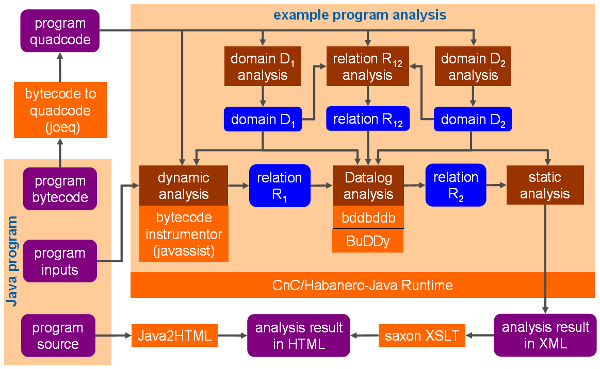
\includegraphics[scale=0.7]{chord_arch.png}}
\htmlonly{{\htmlimg{chord_arch.png}}}
\caption{Architecture of Chord}
\end{label}
\end{center}
\end{figure}

{\bf Under Construction}

%\section{Inputs}
%The inputs to Chord are:
%\begin{itemize}
%\item
%Various system properties dictating the desired configuration and functionality of Chord.
%Chapter \ref{chap:properties} describes how to set properties and the meaning of properties
%recognized by Chord.
%\item
%A Java program to be analyzed.  The program is specified in terms of the main class of the program (via property \code{chord.main.class}) and the application classpath of the program (via property \code{chord.class.path}).  These two properties suffice if only static analysis will be performed; if dynamic analysis is desired, then command-line arguments to run the program must also be provided (via property \code{chord.args}).  Chord analyzes Java bytecode, not source code; however, if it is desired to present analysis results at the Java source level, then the Java source path of the program must also be provided (via property \code{chord.src.path}).
%\end{itemize}
%
%\section{Chord Project}
%project: classic or modern
%analyses determined by ...
%\section{Program Analyses}
%dynamic analysis: \ref{chap:dynamic-analysis}
%Datalog analysis: \ref{chap:datalog-analysis}
%\section{Outputs}


\chapter{Chord Properties}
\label{chap:properties}

The only way to specify inputs to Chord is by means of system properties.
There is no command-line argument processing in Chord and any command-line arguments are ignored.
Section \ref{sec:properties-setting} explains how to set properties and
Section \ref{sec:properties-meaning} explains the meaning of properties recognized by Chord.

\section{How to Set Properties}
\label{sec:properties-setting}

A property can be passed to Chord in any of several ways.
The reason for providing multiple ways is to provide users shorthand ways for defining properties
once and for all for a particular input Java program, or even once and for all across all Chord runs. 
The following are the different ways by which a property can be passed to Chord in decreasing order of precedence:

\begin{enumerate}
\item

On the command-line via the \code{-D<key>=<value>} format.

Use this option to specify properties specific to the current run of Chord.

Typical usage of this option is by running the following command in Chord's \code{main/} directory:
\begin{verbatim}
    prompt> ant -D<key1>=<value1> ... -D<keyN>=<valueN> run
\end{verbatim}

\item

Via the file specified by property \code{chord.props.file}.

Use this option to specify once and for all properties of the program to
be analyzed (e.g., property \code{chord.main.class} specifying the name of that program's main class, property \code{chord.class.path}
specifying the application classpath of that program, etc.).

The default value of this property is \code{[chord.work.dir]/chord.properties} and typically
does not need to be changed by users.
Property \code{chord.work.dir} specifies the directory in which Chord will run.
The default value of this property is the current directory but users must typically set
it on the command line, as follows:

\begin{verbatim}
    prompt> ant -Dchord.work.dir=<...> run
\end{verbatim}
where \code{<...>} denotes the absolute or relative path of the top-level directory of
the program to be analyzed, which contains a file named \code{chord.properties} that users
must create themselves and populate with properties that are recognized by chord and
are specific to that program.

\item

Via file \code{main/chord.properties}.

Use this option to specify once and for all properties you would like to hold in every run of Chord
(e.g., property \code{chord.max.heap} specifying the maximum heap memory size to be used by the
JVM running Chord).
\end{enumerate}

\section{Meaning of Properties}
\label{sec:properties-meaning}

The following properties are recognized by Chord.
The separator for list-valued properties can be either a blank space, a comma, a colon, or a semi-colon.
Notation {\tt [<...>]} is used in this section to denote the value of the property named {\tt <...>}.

\subsection{Java Program Properties} 
\label{sec:program-props}

This section describes properties of the Java program to be analyzed, such as
its main class, the location(s) of its class files and Java source
files, and command-line arguments to be used when running the program.

\code{chord.work.dir}
\begin{quote}
{\bf Type:} location \\
{\bf Description:} Working directory during Chord's execution.  This is
usually the top-level directory of the input Java program. \\
{\bf Default value:} current working directory
\end{quote}

\code{chord.props.file}
\begin{quote}
{\bf Type:} location \\
{\bf Description:} Properties file loaded by Chord at the
beginning before doing anything else.  Any of the below properties may
be defined in this file to avoid defining them on the command line
(using the \code{-D<key>=<value>} format) every time Chord is run.
Each relative file/directory name in the value of any property defined
in this file is treated relative to Chord's working directory (which
is specified by property \code{chord.work.dir}). \\
{\bf Default value:} \code{[chord.work.dir]/chord.properties}
\end{quote}

\code{chord.main.class}
\begin{quote}
{\bf Type:} class \\
{\bf Description:} Fully-qualified name of the main class of the input Java program (e.g., \code{com.example.Main}).
\end{quote}

\code{chord.class.path}
\begin{quote}
{\bf Type:} path \\
{\bf Description:} Classpath of the input Java program.  It does not need to include
boot classes (i.e., classes in \code{[sun.boot.class.path]}) or
standard extensions (i.e., classes in jar files in directory \code{[java.home]/lib/ext/}). \\
{\bf Default value:} {\tt ""}
\end{quote}

\code{chord.src.path}
\begin{quote}
{\bf Type:} path \\
{\bf Description:} Source path of the input Java program. \\
{\bf Default value:} {\tt ""} \\
{\bf Note:} Chord analyzes only Java bytecode, not Java source code.  This property is used only by the task of converting Java source files into HTML files by analyses that need to present their results at the Java source code level (by calling method \code{chord.program.Program.g().HTMLizeJavaSrcFiles())}.
\end{quote}

\code{chord.run.ids}
\begin{quote}
{\bf Type:} string list \\
{\bf Description:} List of IDs to identify runs of the input Java program. \\
{\bf Default value:} {\tt 0} \\
{\bf Note:} This property is used only when Chord runs the input Java program, namely, when it is asked to compute the analysis scope dynamically (i.e., when \code{[chord.scope.kind]=dynamic}) or when it is asked to run a dynamic analysis. 
\end{quote}

\code{chord.args.<id>}
\begin{quote}
{\bf Type:} string \\
{\bf Description:} Command-line arguments string to be used for the input Java program in the run having ID {\tt <id>}. \\
{\bf Default value:} {\tt ""} \\
{\bf Note:} This property is used only when Chord runs the input Java program, namely, when it is asked to compute the analysis scope dynamically (i.e., when \code{[chord.scope.kind]=dynamic}) or when it is asked to run a dynamic analysis.
\end{quote}

\code{chord.runtime.jvmargs}
\begin{quote}
{\bf Type:} string \\
{\bf Description:} Arguments to JVM which runs the input Java program. \\
{\bf Default value:} {\tt "-ea -Xmx1024m"} \\
{\bf Note:} This property is used only when Chord runs the input Java program, namely, when it is asked to compute the analysis scope dynamically (i.e., when \code{[chord.scope.kind]=dynamic}) or when it is asked to run a dynamic analysis. 
\end{quote}

\subsection{Analysis Scope Properties}
\label{sec:scope-props}

This section describes properties that specify how the analysis scope of the input Java program is computed.
See Chapter \ref{chap:computing-scope} for more details.

\code{chord.scope.kind}
\begin{quote}
{\bf Type:} {\tt [dynamic|rta|cha]} \\
{\bf Description:} Algorithm to compute analysis scope.  The choices are {\tt dynamic} (dynamic analysis), {\tt rta} (Rapid Type Analysis), and {\tt cha} (Class Hierarchy Analysis). \\
{\bf Default value:} {\tt rta} \\
{\bf Note:} This property is ignored if property \code{chord.reuse.scope} is set to {\tt true} and the files specified by properties \code{chord.methods.file} and \code{chord.reflect.file} exist. 
\end{quote}

\code{chord.reflect.kind}
\begin{quote}
{\bf Type:} {\tt [none|dynamic|static|static\_cast]} \\
{\bf Description:} Algorithm to resolve reflection.  The choices are {\tt none} (do not resolve any reflection),
{\tt dynamic} (run the program and observe how reflection is resolved),
{\tt static} (resolve reflection statically but without analyzing casts), and
{\tt static\_cast} (resolve reflection statically by analyzing casts). \\
{\bf Default value:} {\tt none}
\end{quote}

\code{chord.ch.kind}
\begin{quote}
{\bf Type:} {\tt [static|dynamic]} \\
{\bf Description:} Algorithm to build the class hierarchy.  If it is {\tt dynamic}, then the input Java program is executed
and classes not loaded by the JVM while running the program are excluded while building the class hierarchy. \\
{\bf Default value:} {\tt static} \\
{\bf Note:} This property is relevant only if \code{chord.scope.kind} is {\tt cha} since only this
scope computing algorithm queries the class hierarchy. 
\end{quote}

\code{chord.ssa}
\begin{quote}
{\bf Type:} bool  \\
{\bf Description:} Do SSA (Static Single Assignment) transformation of the bodies of all methods deemed reachable by the algorithm used to compute analysis scope. \\
{\bf Default value:} {\tt true}
\end{quote}

% TODO: mention that below two properties are also used by instrumentor to decide which classes to exclude from instrumentation

\code{chord.std.scope.exclude}
\begin{quote}
{\bf Type:} string list \\
{\bf Description:} Partial list of prefixes of names of classes, typically inside the JDK standard library, whose methods must be treated as no-ops. \\
{\bf Default value:} {\tt ""}
\end{quote}

\code{chord.ext.scope.exclude}
\begin{quote}
{\bf Type:} string list \\
{\bf Description:} Partial list of prefixes of names of classes, typically outside the JDK standard library, whose methods must be treated as no-ops. \\
{\bf Default value:} {\tt ""}
\end{quote}

\code{chord.scope.exclude}
\begin{quote}
{\bf Type:} string list \\
{\bf Description:} Complete list of prefixes of names of classes whose methods must be treated as no-ops. \\
{\bf Default value:} \code{"[chord.std.scope.exclude],[chord.ext.scope.exclude]"}
\end{quote}

\code{chord.std.check.exclude}
\begin{quote}
{\bf Type:} string list \\
{\bf Description:} Partial list of prefixes of names of classes, typically inside the JDK standard library, to be excluded by analyses.  Interpretation of this property is analysis-specific. \\
{\bf Default value:} \code{"java.,javax.,sun.,com.sun.,com.ibm.,} \code{org.apache.harmony."}
\end{quote}

\code{chord.ext.check.exclude}
\begin{quote}
{\bf Type:} string list \\
{\bf Description:} Partial list of prefixes of names of classes, typically outside the JDK standard library, to be excluded by analyses.  Interpretation of this property is analysis-specific. \\
{\bf Default value:} {\tt ""}
\end{quote}

\code{chord.check.exclude}
\begin{quote}
{\bf Type:} string list \\
{\bf Description:} Complete list of prefixes of names of classes to be excluded by analyses.  Interpretation of this property is analysis-specific. \\
{\bf Default value:} \code{"[chord.std.check.exclude],[chord.ext.check.exclude]"}
\end{quote}

\subsection{Functionality Properties}
\label{sec:func-props}

This section describes properties that dictate what task(s) Chord must perform.

\code{chord.build.scope}
\begin{quote}
{\bf Type:} bool \\
{\bf Description:} Compute the analysis scope of the input Java program using the algorithm. \\
{\bf Default value:} {\tt false} \\
{\bf Note:} The analysis scope is computed regardless of the value of this property if another task (e.g., an analysis specified via property \code{chord.run.analyses}) demands it.
\end{quote}

\code{chord.run.analyses}
\begin{quote}
{\bf Type:} string list  \\
{\bf Description:} List of names of analyses to be run in order. \\
{\bf Default value:} {\tt ""} \\
{\bf Note:} If the analysis is written in Java, its name is specified via statement {\tt name=<...>} in its {\tt @Chord} annotation.  If the analysis is written in Datalog, its name is specified via a line of the form ``{\tt \# name=<...>}".
\end{quote}

\code{chord.print.methods}
\begin{quote}
{\bf Type:} string list  \\
{\bf Description:} List of methods whose intermediate representation to print to standard output. \\
{\bf Default value:} {\tt ""} \\
{\bf Note:} Specify each method in format \code{<mname>:<mdesc>@<cname>} where {\tt <mname>} is the method's name, {\tt <mdesc>} is the method's descriptor, and {\tt <cname>} is the name of the method's declaring class. In {\tt <cname>}, use `.' instead of `/', and use {\tt \#} instead of the dollar character. 
\end{quote}

\code{chord.print.classes}
\begin{quote}
{\bf Type:} string list  \\
{\bf Description:} List of classes whose intermediate representation to print to standard output. \\
{\bf Default value:} {\tt ""} \\
{\bf Note:} In class names, use `.' instead of `/', and use {\tt \#} instead of the dollar character. 
\end{quote}

\code{chord.print.all.classes}
\begin{quote}
{\bf Type:} bool \\
{\bf Description:} Print intermediate representation of all classes in scope to standard output. \\
{\bf Default value:} {\tt false}
\end{quote}

\code{chord.print.rels}
\begin{quote}
{\bf Type:} string list  \\
{\bf Description:} List of names of program relations whose contents must be printed to files \code{[chord.out.dir]/<...>.txt} where {\tt <...>} denotes the relation name. \\
{\bf Default value:} {\tt ""} \\
{\bf Note:} This functionality must be used with caution as certain program relations, albeit represented compactly as BDDs, may contain a large number (e.g., millions) of tuples, resulting in voluminous output when printed in explicit form to a text file.  See Section \ref{sec:tuning-datalog-analysis} for a more efficient way to query the contents of program relations (namely, by using the {\tt debug} target provided in file {\tt build.xml} in Chord's \code{main/} directory).
\end{quote}

\code{chord.print.project}
\begin{quote}
{\bf Type:} bool \\
{\bf Description:} Create files \code{targets_sortby_name.html}, \code{targets_sortby_kind.html}, and \code{targets_sortby_producers.html} in directory \code{[chord.out.dir]}, publishing all tasks and targets defined by analyses in paths \code{[chord.java.analysis.path]} and \code{[chord.dlog.analysis.path]}.  \\
{\bf Default value:} {\tt false}
\end{quote}

\code{chord.print.results}
\begin{quote}
{\bf Type:} bool \\
{\bf Description:} Print the results of analyses in HTML.  Interpretation of this property is analysis-specific.  \\
{\bf Default value:} {\tt true}
\end{quote}

\code{chord.verbose}
\begin{quote}
{\bf Type:} int in the range [0..5]  \\
{\bf Description:} Control the verbosity of messages during Chord's execution.  \\
{\bf Default value:} {\tt 1}
\end{quote}

\subsection{Project Properties}
\label{sec:project-props}

This section describes properties regarding analyses executed by Chord.

\code{chord.classic}
\begin{quote}
{\bf Type:} bool \\
{\bf Description:} Whether to use the classic project (as opposed to the modern project).  See Chapter\ref{chap:analyses} for the difference between the two kinds of projects. \\
{\bf Default value:} \code{true}
\end{quote}

\code{chord.std.java.analysis.path}
\begin{quote}
{\bf Type:} path \\
{\bf Description:} Partial classpath of analyses written in Java (i.e., {\tt @Chord}-annotated classes).
Conventionally, it includes all such analyses that are predefined in Chord.  \\
{\bf Default value:} The absolute path of file \code{chord.jar}
\end{quote}

\code{chord.ext.java.analysis.path}
\begin{quote}
{\bf Type:} path \\
{\bf Description:} Partial classpath of analyses written in Java (i.e., {\tt @Chord}-annotated classes).
Conventionally, it includes all such external analyses that users want to run. \\
{\bf Default value:} {\tt ""}
\end{quote}

\code{chord.java.analysis.path}
\begin{quote}
{\bf Type:} path \\
{\bf Description:} Complete classpath of analyses written in Java (i.e., {\tt @Chord}-annotated classes). \\
{\bf Default value:} \code{[chord.std.java.analysis.path]:[chord.ext.java.analysis.path]}
\end{quote}

\code{chord.std.dlog.analysis.path}
\begin{quote}
{\bf Type:} path \\
{\bf Description:} Partial classpath of analyses written in Datalog (i.e., files with suffix {\tt .dlog} or {\tt .datalog}).
Conventionally, it includes all such analyses that are predefined in Chord.  \\
{\bf Default value:} The absolute path of file \code{chord.jar}
\end{quote}

\code{chord.ext.dlog.analysis.path}
\begin{quote}
{\bf Type:} path \\
{\bf Description:} Partial classpath of analyses written in Datalog (i.e., files with suffix {\tt .dlog} or {\tt .datalog}).
Conventionally, it includes all such external analyses that users want to run. \\
{\bf Default value:} {\tt ""}
\end{quote}

\code{chord.dlog.analysis.path}
\begin{quote}
{\bf Type:} path  \\
{\bf Description:} Complete classpath of analyses written in Datalog (i.e., files with suffix {\tt .dlog} or {\tt .datalog}). \\
{\bf Default value:} \code{[chord.std.dlog.analysis.path]:[chord.ext.dlog.analysis.path]}
\end{quote}

\subsection{Instrumentation Properties}
\label{sec:instr-props}

This section describes properties regarding bytecode instrumentation and dynamic analysis.

% TODO: mention chord.scope.exclude* here
\code{chord.use.jvmti}
\begin{quote}
{\bf Type:} bool \\
{\bf Description:} Whether the JVMTI-based bytecode instrumentation agent from \code{main/agent/} must be used for running dynamic analyses. \\
{\bf Default value:} \code{false}
\end{quote}

\code{chord.instr.kind}
\begin{quote}
{\bf Type:} {\tt [offline|online]}  \\
{\bf Description:} The kind of bytecode instrumentation.  The choices are offline and online (load-time).  \\
{\bf Default value:} {\tt offline}
\end{quote}

\code{chord.trace.kind}
\begin{quote}
{\bf Type:} {\tt [full|pipe]}  \\
{\bf Description:} The medium by which an event-generating JVM and an event-handling JVM communicate in a dynamic analysis.  The choices are regular file and POSIX pipe.  \\
{\bf Default value:} {\tt full} 
\end{quote}

\code{chord.trace.block.size}
\begin{quote}
{\bf Type:} int \\
{\bf Description:} Number of bytes to read/write in a single operation from/to the event trace file in a multi-JVM dynamic analysis. \\
{\bf Default value:} {\tt 4096}
\end{quote}

\code{chord.dynamic.haltonerr}
\begin{quote}
{\bf Type:} bool \\
{\bf Description:} Whether to terminate Chord if the input Java program terminates abnormally during dynamic analysis. \\
{\bf Default value:} true
\end{quote}

\code{chord.dynamic.timeout}
\begin{quote}
{\bf Type:} int  \\
{\bf Description:} The amount of time, in milliseconds, after which to kill the process running the given program during dynamic analysis, or -1 if the process must never be killed. \\
{\bf Default value:} {\tt -1}
\end{quote}

\code{chord.max.cons.size}
\begin{quote}
{\bf Type:} int \\
{\bf Description:} Maximum number of bytes over which events generated during the execution of any constructor in the given program may span. \\
{\bf Default value:} {\tt 50000000} \\
{\bf Note:} This property is relevant only for dynamic analyses which want events of the form {\tt BEF\_NEW} $h$ $t$ $o$ to be generated (see Section \ref{sec:instr-events}).  The problem with generating such events at run-time is that the ID $o$ of the object freshly created by thread $t$ at object allocation site $h$ cannot be instrumented until the object is fully initialized (i.e., its constructor has finished executing).  Hence, Chord first generates a ``crude dynamic trace", which has events of the form {\tt BEF\_NEW} $h$ $t$ and {\tt AFT\_NEW} $h$ $t$ $o$ generated before and after the execution of the constructor, respectively.  A subsequent pass generates a ``final dynamic trace", which replaces each {\tt BEF\_NEW} $h$ $t$ event by {\tt BEF\_NEW} $h$ $t$ $o$.  For this purpose, however, Chord must buffer all events generated between the {\tt BEF\_NEW} and {\tt AFT\_NEW} events, and this property specifies the number of bytes over which these events may span.  If the actual number of bytes exceeds the value specified by this property (e.g., if the constructor throws an exception and the {\tt AFT\_NEW} event is not generated at all), then Chord simply generates event {\tt BEF\_NEW} $h$ $i$ $0$ (i.e., it treats the created object as having ID 0, which is the ID also used for {\tt null}). 
\end{quote}

\subsection{Caching Properties}
\label{sec:caching-props}

This section describes properties that specify what must be reused by Chord, if available, from previous runs instead of recomputing.

\code{chord.reuse.scope}
\begin{quote}
{\bf Type:} bool \\
{\bf Description:} Compute analysis scope using the information in files specified by properties \code{chord.methods.file} and \code{chord.reflect.file}, if both of those files exist. \\
{\bf Default value:} {\tt false} \\
{\bf Note:} Property \code{chord.scope.kind} is ignored if this property is set to {\tt true} and the two files exist. 
\end{quote}

\code{chord.reuse.rels}
\begin{quote}
{\bf Type:} bool  \\
{\bf Description:} Load each desired program relation named \code{<name>} from the BDD stored in file \code{[chord.bddbddb.work.dir]/<name>.bdd}, if the file exists. \\
{\bf Default value:} {\tt false}
\end{quote}

\code{chord.reuse.traces}
\begin{quote}
{\bf Type:} bool \\
{\bf Description:} Reuse event traces stored in file(s) \code{chord.trace.file]_full_ver0_runM.txt} for dynamic analysis, if those files exist,
where \code{M} ranges over run IDs specified by property \code{chord.run.ids}.
Property \code{chord.trace.kind} must be set to {\tt full} if this property is set to {\tt true}. \\
{\bf Default value:} {\tt false}
\end{quote}

\subsection{Chord JVM Properties}
\label{sec:jvm-props}

This section describes properties regarding the JVM that runs Chord.

\code{chord.max.heap}
\begin{quote}
{\bf Type:} string \\
{\bf Description:} Maximum heap memory size of the JVM running Chord. \\
{\bf Default value:} {\tt 1024m}
\end{quote}

\code{chord.max.stack}
\begin{quote}
{\bf Type:} string \\
{\bf Description:} Maximum thread stack size of the JVM running Chord. \\
{\bf Default value:} {\tt 32m}
\end{quote}

\code{chord.jvmargs}
\begin{quote}
{\bf Type:} string \\
{\bf Description:} Arguments to the JVM running Chord. \\
{\bf Default value:} \code{"-showversion} \code{-ea} \code{-Xmx[chord.max.heap]} \code{-Xss[chord.max.stack]"}
\end{quote}

\subsection{BDD Properties}
\label{sec:bdd-props}

This section describes properties concerning BDD-based Datalog solver bddbddb that is used by Chord to run analyses written in Datalog.

\code{chord.use.buddy}
\begin{quote}
{\bf Type:} bool \\
{\bf Description:} Whether BDD library BuDDy from \code{main/bdd/} must be used by bddbddb. \\
{\bf Default value:} \code{false}
\end{quote}

\code{chord.bddbddb.max.heap}
\begin{quote}
{\bf Type:} string \\
{\bf Description:} Maximum heap memory size of JVM running bddbddb. \\
{\bf Default value:} {\tt 1024m} \\
{\bf Note:} bddbddb is invoked in a separate JVM for each analysis written in Datalog that is executed.
This is primarily because multiple Datalog analyses may be executed in a single run of Chord,
resulting in multiple invocations of bddbddb, and it is difficult to reset the state of bddbddb on each invocation. 
\end{quote}

\subsection{Output Location Properties}
\label{sec:output-props}

This section describes properties specifying the names of files and directories output by Chord.
Most users will not need to alter the default values of these properties.

\code{chord.out.file}
\begin{quote}
{\bf Type:} location \\
{\bf Description:} Absolute location of the file to which the standard output stream is redirected during Chord's execution. \\
{\bf Default value:} \code{null}
\end{quote}

\code{chord.err.file}
\begin{quote}
{\bf Type:} location  \\
{\bf Description:} Absolute location of the file to which the standard error stream is redirected during Chord's execution. \\
{\bf Default value:} \code{null}
\end{quote}

\code{chord.out.dir}
\begin{quote}
{\bf Type:} location \\
{\bf Description:} Absolute location of the directory to which Chord dumps all files. \\
{\bf Default value:} \code{[chord.work.dir]/chord_output/}
\end{quote}

\code{chord.reflect.file}
\begin{quote}
{\bf Type:} location  \\
{\bf Description:} Absolute location of the file from/to which resolved reflection information is read/written. \\
{\bf Default value:} \code{[chord.out.dir]/reflect.txt}
\end{quote}

\code{chord.methods.file}
\begin{quote}
{\bf Type:} location  \\
{\bf Description:} Absolute location of the file from/to which list of methods deemed reachable is read/written. \\
{\bf Default value:} \code{[chord.out.dir]/methods.txt}
\end{quote}

\code{chord.classes.file}
\begin{quote}
{\bf Type:} location  \\
{\bf Description:} Absolute location of the file from/to which list of classes deemed reachable is read/written.  \\
{\bf Default value:} \code{[chord.out.dir]/classes.txt}
\end{quote}

\code{chord.bddbddb.work.dir}
\begin{quote}
{\bf Type:} location \\
{\bf Description:} Absolute location of the directory used by BDD-based Datalog solver bddbddb as its input/output directory (namely, for program domain files {\tt *.dom} and {\tt *.map}, and program relation files {\tt *.bdd}). \\
{\bf Default value:} \code{[chord.out.dir]/bddbddb/}
\end{quote}

\code{chord.boot.classes.dir}
\begin{quote}
{\bf Type:} location \\
{\bf Description:} Absolute location of the directory from/to which instrumented classes of the input Java program inside the JDK standard library are read/written by dynamic analyses. \\
{\bf Default value:} \code{[chord.out.dir]/boot_classes/}
\end{quote}

\code{chord.user.classes.dir}
\begin{quote}
{\bf Type:} location  \\
{\bf Description:} Absolute location of the directory from/to which instrumented classes of the input Java program outside the JDK standard library are read/written by dynamic analyses. \\
{\bf Default value:} \code{[chord.out.dir]/user_classes/}
\end{quote}

\code{chord.instr.scheme.file}
\begin{quote}
{\bf Type:} location \\
{\bf Description:} Absolute location of the file specifying the kind and format of events in trace files used by dynamic analyses. \\
{\bf Default value:} \code{[chord.out.dir]/scheme.ser}
\end{quote}

\code{chord.trace.file}
\begin{quote}
{\bf Type:} location  \\
{\bf Description:} Absolute location of trace files used by dynamic analyses. \\
{\bf Default value:} \code{[chord.out.dir]/trace} \\
{\bf Note:} Suffix \code{_full_verN.txt} or \code{_pipe_verN.txt} is appended to the name of the file, depending upon whether it is a regular file or a POSIX pipe, respectively, where {\tt N} is the version of the file (multiple versions are maintained if the trace is transformed by filters defined by the dynamic analysis; 0 is the final version).  If \code{chord.reuse.traces} is set to {\tt true}, then \code{_full_verN_runM.txt} is appended to the name of the file, where {\tt M} is the run ID. 
\end{quote}

%\item
%\code{chord.main.dir}
% location
%Absolute location of the {\tt main/} directory in Chord's installation.

%\item
%\code{chord.save.maps}
% bool
%Write to file \code{[chord.bddbddb.work.dir]/<...>.map} when saving program domain named {\tt <...>}.
%{\tt true}
%{\bf Note:} This functionality is useful for debugging Datalog programs using the {\tt debug} target provided in file {\tt build.xml} in Chord's {\tt main/} directory (see Section \ref{sec:tuning-datalog-analysis}).


\chapter{Predefined Analyses}
\label{chap:predefined-analyses}

This chapter describes various predefined analyses in Chord.

\section{Static Datarace Analysis}

To run Chord's static datarace analysis, run the following
command in Chord's {\tt main/} directory:

\begin{verbatim}
    prompt> ant -Dchord.work.dir=<...> -Dchord.run.analyses=datarace-java run
\end{verbatim}

where {\tt <...>} denotes the absolute or relative path of a directory
containing a file named \code{chord.properties} which defines
properties \code{chord.main.class}, \code{chord.class.path}, and
\code{chord.src.path}.  See Chapter \ref{chap:properties} for the
meaning of these properties.

Directory \code{main/examples/datarace_test/} provides a toy Java
program on which you can run the datarace analysis.  First run {\tt
  ant} in that directory (in order to compile the program's {\tt
  .java} files to {\tt .class} files) and then run the above command
in Chord's {\tt main/} directory with {\tt <...>} replaced by
\code{examples/datarace_test/}.  Upon successful completion, the
following files should be produced in directory
\code{examples/datarace_test/chord_output/}:

\begin{itemize}
\item
File \code{dataraces_by_fld.html}, listing all dataraces grouped by
the field on which they occur; all dataraces on the same instance
field or the same static field are listed in the same group, and so
are all dataraces on array elements.
\item
File \code{dataraces_by_obj.html}, listing all dataraces grouped by
the abstract object on whose field they occur; dataraces on all static
fields are listed in the same group, and so are dataraces on different
instance fields of the same abstract object.
\end{itemize}

\section{Static Deadlock Analysis}

To run Chord's static deadlock analysis,  run the following
command in Chord's {\tt main/} directory:

\begin{verbatim}
    prompt> ant -Dchord.work.dir=<...> -Dchord.run.analyses=deadlock-java run
\end{verbatim}

where {\tt <...>} denotes the absolute or relative path of a directory
containing a file named \code{chord.properties} which defines
properties \code{chord.main.class}, \code{chord.class.path}, and
\code{chord.src.path}.  See Chapter \ref{chap:properties} for the
meaning of these properties.

Directory \code{main/examples/deadlock_test/} provides a toy Java
program on which you can run the deadlock analysis.  First run {\tt
  ant} in that directory (in order to compile the program's {\tt
  .java} files to {\tt .class} files) and then run the above command
in Chord's {\tt main/} directory with {\tt <...>} replaced by
\code{examples/deadlock_test/}.  Upon successful completion, the
file \code{deadlocks.html} should be produced in directory
\code{examples/deadlock_test/chord_output/}.

\section{May-Alias and Call-Graph Analyses}

TODO

\chapter{Writing and Running Analyses}
\label{chap:analyses}

Chord is built around the notion of modeling a program with relations.
A Chord analysis is a program component that operates on these relations.
It may consume zero or more relations, do some work on them, and then output zero or more relations.
It may also print output in some other format, perhaps human-readable text or HTML.
``Relation'' here has the same meaning it does in the context of relational databases: a set of tuples, containing elements of one or more domains.  
%For example, the relation \texttt{reachableM(m:M)} identifies a subset of 


An analysis can be written in one of two ways: either as a Java class or as a datalog program. 

\section{Dependency information}

Chord has two kinds of projects: ``Classic'' and ``Modern''.  Despite the names, classic is effectively the standard at this point.
In the classic model, each analysis specifies the domains/relations it consumes and that it produces.
This defines an implicit dependency graph between analyses.  For a datalog analysis, the ``input'' and ``output'' keywords on relations specify the requirements and results of an analysis.  For a Java analysis, the \texttt{@Chord} annotation does so. 

\section{Domains}

In Chord, a domain is represented as a list of possible values. 
The value types must be comparable and hashable.
Strings work, as do integers, \texttt{joeq} quads, fields, types, and so forth. 
%
% What are the required types?

Both domains and relations have names. The built-in relations are usually identified by a single capital letter.
Chord by default includes code for constructing a number of domains.

It is sometimes useful to construct new domains in the middle of an analysis, perhaps as a way of compactly describing some entities that required nontrivial work to find. Domains, for now, must be defined in Java. One key requirement is that construction must be deterministic: if the elements in a domain can be reordered from execution to execution on the same program, this can result in subtle and hard-to-track-down bugs.


\begin{itemize}
\item
B is the domain of basic blocks.
\item
C is the domain of abstract calling contexts.
\item
E is the domain of program points that read or write a field.
\item
F is the domain of fields inside a class.
\item
H is the domain of allocation sites.
\item
I is the domain of invocation statements (method calls)
\item
L is the domain of lock acquisition points.
\item
M is the domain of program methods.
\item
P is the domain of simple statements. %SAY MORE HERE?
\item
R is the domain of lock release points.
\item
T is the domain of types (classes and primitives).
\item
V is the domain of reference-typed variables.
\item
W is the domain of loop head statements. %SAY MORE HERE?
\item
Z is a domain of integers corresponding to argument positions.The size of the domain is chosen to 
accommodate the method with the greatest number of arguments.
\item
ZZ is another domain of integers, this one of fixed size and available for other uses.
\end{itemize}

\section{Core relations}

Chord includes code to build a very large number of relations. These standard relations
are very useful in writing your own analyses.
For example, relation \texttt{sub} includes all pairs of types \texttt{(t1, t2)} where \texttt{t2} is a subclass of \texttt{t1}.
Most of these standard relations are in the package \texttt{chord.rels}.

\section{Java analyses}

A Java analysis should extend JavaAnalysis or ProgramRel.  It's usually easiest if an analysis
only produces one relation, in which case extending ProgramRel is the best approach.
If you extend ProgramRel, all the work of creating and saving the relation is taken care of for you;
all you need to do is add tuples to the relation.Typically you do this by calling
\texttt{super.add(...)} with the tuple you wish to add to the relation.
For forther convenience, you can implement one of the Visitor interfaces defined in 
\texttt{chord.program.visitors}.  This will force you to implement some \texttt{visit} methods that iterate over
all elements in some domain, such as all methods or all invocation points. 

Sometimes, you need to create two different relations at the same time. In this case, the right approach is to
extend JavaAnalysis, and explicitly create and save the relations on your own.
\textbf{Should reference JavaDoc.  Should make sure JavaDoc explains what you need to do to fill and save a relation}.

Regardless of which of these approaches you take, every Java analysis must have an \texttt{@Chord} annotation.
This annotation is a set of named fields.
At a minimum, this annotation must specify the name of the analysis.
If you extend ProgramRel, the name of the analysis will be treated as the same as that of the generated relation.
For example, \texttt{@Chord(name = "F")} is a valid annotation. 
The name of the Java class that generates the relation is ignored by Chord -- only the annotation matters.

\textbf{MAYUR, IS SIGN MANDATORY?   IF NOT, WHEN CAN IT BE OMITTED?}

There are also other annotation fields available.
You may specify the dependencies of your analysis via \texttt{consumes = \{ "xyz"\}}.

If your analysis does not extend ProgramRel, you should also specify the relations that your 
analysis produces. You do this via the \texttt{produces} relation.

%Should mention the signs fields.
%
%

The default value of property \code{chord.java.analysis.path}
is \code{chord.std.java.analysis.path}:\code{chord.ext.java.analysis.path},
where the defalt value of \code{chord.std.java.analysis.path} is the location of file \code{chord.jar}, and
the default value of \code{chord.ext.java.analysis.path} is empty (users defining their own Java analyses are expected to
set the latter property).

The default value of property \code{chord.dlog.analysis.path}
is \code{chord.std.dlog.analysis.path}:\code{chord.ext.java.analysis.path},
where the defalt value of \code{chord.std.java.analysis.path} is the location of file \code{chord.jar}, and
the default value of \code{chord.ext.java.analysis.path} is empty (users defining their own Java analyses are expected to
set the latter property).

\section{Running an Analysis}
\label{sec:running-analysis}

Running a Chord analysis is straightforward.
The property  \texttt{chord.run.analyses} is a list of analyses to be run. Chord will compute the listed dependencies for each of these relations and run these prerequisites before running the analysis you specify.

Chord has two kinds of projects: ``Classic'' and ``Modern''.  Despite the names, classic is effectively the standard at this point.
In the classic model, there is an implicit dependency graph between analyses. For a datalog analysis (program), the ``input'' and ``output'' keywords in defining a relation specify the requirements and outputs of an analysis.  For a Java analysis, the \texttt{@Chord} annotation does so. See the section ``writing a Java analysis'' for details.

\texttt{chord.print.rels} is a list of relations to dump to disk. Note that these relations are printed in a somewhat unfriendly format; this is more useful for debugging than for interpreting programs. Note also that listing a relation here does not cause it to be computed; you will get an error at the end of your Chord execution if you ask it to print a relation that has not been computed.

%List of names of program analyses to be run in order.
%chord.java.analysis.path    path    Classpath containing program analyses in Java (i.e. @Chord-annotated classes). ${chord.main.dir}/classes/
%chord.dlog.analysis.path    path    Path of directories containing program analyses in Datalog (i.e. *.datalog and *.dlog files).  ${chord.main.dir}/src/main/dlog/
%chord.reuse.rels    bool    Construct program relations from BDDs stored on disk (from a previous run of Chord) whenever possible instead of re-computing them.    false
%chord.print.results     bool    Print the results of program analyses in HTML. true


\chapter{Dynamic Analysis}
\label{chap:dynamic-analysis}

This chapter describes everything about dynamic analysis in Chord.
Section \ref{sec:writing-dynamic-analysis} describes how to write a dynamic analysis,
Section \ref{sec:running-dynamic-analysis} describes how to compile and run it,
and Section \ref{sec:instr-events} describes common dynamic analysis events
supported in Chord.

\section{Writing a Dynamic Analysis}
\label{sec:writing-dynamic-analysis}

Follow the following steps to write your own dynamic analysis.

Create a class extending \code{chord.project.analyses.DynamicAnalysis} and override
the appropriate methods in it.
The only methods that must be compulsorily overridden are method \code{getInstrScheme()},
which must return an instance of the ``instrumentation scheme" required by
your dynamic analysis (i.e., the kind and format of events to be generated during an
instrumented program's execution)
plus each \code{process<event>(<args>)} method that corresponds to event {\tt <event>}
with format {\tt <args>} enabled by the chosen instrumentation scheme.
See Section \ref{sec:instr-events} for the kinds of supported events and their formats.

A sample such class \code{MyDynamicAnalysis} is shown below:

\begin{verbatim}
    import chord.project.analyses.DynamicAnalysis;
    import chord.instr.InstrScheme;

    // ***TODO***: analysis won't be recognized by Chord without this annotation
    @Chord(name=<name-of-analysis>)    
    public class MyDynamicAnalysis extends DynamicAnalysis {
        InstrScheme scheme;

        @Override
        public InstrScheme getInstrScheme() {
            if (scheme != null)
                return scheme;
            scheme = new InstrScheme();
            // ***TODO***: Choose (<event1>, <args1>), ... (<eventN>, <argsN>)
            // depending upon the kind and format of events required by this
            // dynamic analysis to be generated for this during an instrumented
            // program's execution.
            scheme.set<event1>(<args1>);
            ...
            scheme.set<eventN>(<argsN>);
            return scheme;
        }

        @Override
        public void initAllPasses() {
            // ***TODO***: User code to be executed once and for all
            // before all instrumented program runs start.
        }

        @Override
        public void doneAllPasses() {
            // ***TODO***: User code to be executed once and for all
            // after all instrumented program runs finish.
        }

        @Override
        public void initPass() {
            // ***TODO***: User code to be executed once before each
            // instrumented program run starts.
        }

        @Override
        public void donePass() {
            // ***TODO***: User code to be executed once after each
            // instrumented program run finishes.
        }

        // User-defined event handlers for this dynamic analysis.
        // No-ops if not overridden.
        @Override
        public void process<event1>(<args1>) {
            // ***TODO***: User code for handling events of kind
            // <event1> with format <args1>.
        }
        ...
        @Override
        public void process<eventN>(<argsN>) {
            // ***TODO***: User code for handling events of kind
            // <eventN> with format <argsN>.
        }
    }
\end{verbatim}

\section{Compiling and Running a Dynamic Analysis}
\label{sec:running-dynamic-analysis}

Compile the analysis by placing the directory containing class \code{MyDynamicAnalysis} created
above in the path defined by property \code{chord.ext.java.analysis.path}.

Provide the IDs of program runs to be generated (say 1, 2, ..., M) and the command-line arguments to be
used for the program in each of those runs (say \code{<args1>}, ..., \code{<argsM>}) via properties
\code{chord.run.ids=1,2,...,N} and \code{chord.args.1=<args1>}, ..., \code{chord.args.M=<argsM>}.
By default, \code{chord.run.ids=0} and \code{chord.args.0=""}, that is, the program will be run only
once (using run ID 0) with no command-line arguments.

To run the analysis, set property \code{chord.run.analyses} to \code{<name-of-analysis>}
(recall that \code{<name-of-analysis>} is the name provided in the \code{@Chord} annotation for class
\code{MyDynamicAnalysis} created above).

{\bf Note:} The IBM J9 JVM on Linux is highly recommended if you intend to use Chord for
dynamic program analysis, as it allows you to instrument the entire JDK; using any other
platform will likely require excluding large parts of the JDK from being instrumented.
Additionally, if you intend to use online (load-time) bytecode instrumentation in
your dynamic program analysis, then you will need JDK 6 or higher, since this functionality
requires the \code{java.lang.instrument} API with class retransformation support (the latter
support is available only in JDK 6 and higher).

You can change the default values of various properties for configuring your dynamic analysis;
see Section \ref{sec:scope-props} and Section \ref{sec:instr-props} in Chapter \ref{chap:properties}.
For instance:
\begin{itemize}
\item
You can set property \code{chord.scope.kind} to {\tt dynamic} so that the program scope
is computed dynamically (i.e., by running the program) instead of statically.
\item
You can exclude certain classes (e.g., JDK classes) from being instrumented by setting
properties \code{chord.std.scope.exclude}, \code{chord.ext.scope.exclude}, and
\code{chord.scope.exclude}.
\item
You can choose between online (i.e. load-time) and offline bytecode instrumentation by
setting property \code{chord.instr.kind} to {\tt online} or {\tt offline}.
\item
You can require the event-generating and event-handling JVMs to be one and the same (by setting
property \code{chord.trace.kind} to {\tt none}),
or to be separate (by setting property {\tt chord.trace.kind} to {\tt full} or {\tt pipe}, depending upon
whether you want the two JVMs to exchange events by a regular file or a POSIX pipe, respectively).
Using a single JVM can cause correctness/performance issues if event-handling Java code itself is instrumented
(e.g., say the event-handling code uses class \code{java.util.ArrayList} which is not excluded from program scope).
Using separate JVMs prevents such issues since the event-handling JVM runs uninstrumented bytecode (only
the event-generating JVM runs instrumented bytecode).
If a regular file is used to exchange events between the two JVMs, then the JVMs run serially:
the event-generating JVM first runs to completion, dumps the entire dynamic trace to the regular file,
and then the event-handling JVM processes the dynamic trace.
If a POSIX pipe is used to exchange events between the two JVMs, then the JVMs run in lockstep.
Obviously, a pipe is more efficient for very long traces, but it 
not portable (e.g., it does not currently work on Windows/Cygwin), and the traces cannot be reused
across Chord runs (see the following item).
\item
You can reuse dynamic traces from a previous Chord run by setting property
\code{chord.reuse.traces} to {\tt true}.  In this case, you must also set property
{\tt chord.trace.kind} to {\tt full}.
\item
You can set property \code{chord.dynamic.haltonerr} to {\tt false} to prevent Chord from terminating
even if the program on which dynamic analysis is being performed crashes.
\end{itemize}

Chord offers much more flexibility in crafting dynamic analyses.
You can define your own instrumentor (by subclassing \code{chord.instr.CoreInstrumentor}
instead of using the default \code{chord.instr.Instrumentor}) and your own event handler (by subclassing \code{chord.runtime.CoreEventHandler}
instead of using the default \code{chord.runtime.EventHandler}).
You can ask the dynamic analysis to use your custom instrumentor and/or your custom event handler by overriding
methods \code{getInstrumentor()} and \code{getEventHandler()}, respectively, defined in \code{chord.project.analyses.CoreDynamicAnalysis}.
Finally, you can define your own dynamic analysis template by subclassing \code{chord.project.analyses.CoreDynamicAnalysis}
instead of subclassing the default \code{chord.project.analyses.DynamicAnalysis}.

\section{Common Dynamic Analysis Events}
\label{sec:instr-events}

Chord provides support for instrumenting common dynamic analysis events.
The below table describes these events.

\begin{table}
\begin{center}
\htmlattributes*{table}{border="1" cellpadding="10"}
\begin{tabular}{|l|l|}
\hline
{\bf Event Kind} & {\bf Description} \\
\hline
EnterMainMethod(\bt) & Generated after thread \bt\ enters method \bm\ (index in domain M).
\\
\hline
EnterMethod(\bm, \bt) & Generated after thread \bt\ enters method \bm\ (index in domain M).
\\
\hline
LeaveMethod(\bm, \bt) & Generated before thread \bt\ leaves method \bm\ (index in domain M).
\\
\hline
EnterLoop(\bw, \bt) & Generated before thread \bt\ begins loop \bw\ (index in domain W).
\\
\hline
LoopIteration(\bw, \bt) & Generated before thread \bt\ starts a new iteration of loop \bw\ (index in domain W).
\\
\hline
LeaveLoop(\bw, \bt) & Generated after thread \bt\ finishes loop \bw\ (index in domain W).
\\
\hline
BasicBlock(\bb, \bt) & Generated before thread \bt\ enters basic block \bb\ (index in domain B).
\\
\hline
Quad(\bp, \bt) & Generated before thread \bt\ executes quad at program point \bp\ (index in domain P).
\\
\hline
BefMethodCall(\bi, \bt, \bo) & 
\begin{tabular}{l}
Generated before thread \bt\ executes the method invocation statement at program point \bi\ (index in domain I) with this argument as object \bo. \\
{\bf Note:} This event is not generated before constructor calls; use the BefNew event for that purpose.
\end{tabular}
\\
\hline
AftMethodCall(\bi, \bt, \bo) &
\begin{tabular}{l}
Generated after thread \bt\ executes the method invocation statement at program point \bi\ (index in domain I) with this argument as object \bo. \\
{\bf Note:} This event is not generated after constructor calls; use the AftNew event for that purpose.
\end{tabular}
\\
\hline
BefNew(\bh, \bt, \bo) & Generated before thread \bt\ executes a \code{new} bytecode instruction and allocates fresh object \bo\ at program point \bh\ (index in domain H).
\\
\hline
AftNew(\bh, \bt, \bo) & Generated after thread \bt\ executes a \code{new} bytecode instruction and allocates fresh object \bo\ at program point \bh\ (index in domain H).
\\
\hline
NewArray(\bh, \bt, \bo) & Generated after thread \bt\ executes a \code{newarray} bytecode instruction and allocates fresh object \bo\ at program point \bh\ (index in domain H).
\\
\hline
GetstaticPrimitive(\be, \bt, \bg) & Generated after thread \bt\ reads primitive-typed static field \bg\ (index in domain F) at program point \be\ (index in domain E).
\\
\hline
GetstaticReference(\be, \bt, \bg, \bo) & Generated after thread \bt\ reads object \bo\ from reference-typed static field \bg\ (index in domain F) at program point \be\ (index in domain E).
\\
\hline
PutstaticPrimitive(\be, \bt, \bg) & Generated after thread \bt\ writes primitive-typed static field \bg\ (index in domain F) at program point \be\ (index in domain E).
\\
\hline
PutstaticReference(\be, \bt, \bg, \bo) & Generated after thread \bt\ writes object \bo\ to reference-typed static field \bg\ (index in domain F) at program point \be\ (index in domain E).
\\
\hline
GetfieldPrimitive(\be, \bt, \bb, \bg) & Generated after thread \bt\ reads primitive-typed instance field \bg\ (index in domain F) of object \bb\ at program point \be\ (index in domain E).
\\
\hline
GetfieldReference(\be, \bt, \bb, \bg, \bo) & Generated after thread \bt\ reads object \bo\ from reference-typed instance field \bg\ (index in domain F) of object \bb\ at program point \be\ (index in domain E).
\\
\hline
PutfieldPrimitive(\be, \bt, \bb, \bg) & Generated after thread \bt\ writes primitive-typed instance field \bg\ (index in domain F) of object \bb\ at program point \be\ (index in domain E).
\\
\hline
PutfieldReference(\be, \bt, \bb, \bg, \bo) & Generated after thread \bt\ writes object \bo\ to reference-typed instance field \bg\ (index in domain F) of object \bb\ at program point \be\ (index in domain E).
\\
\hline
AloadPrimitive(\be, \bt, \bb, \bi) & Generated after thread \bt\ reads the primitive-typed element at index \bi\ of array object \bb\ at program point \be\ (index in domain E).
\\
\hline
AloadReference(\be, \bt, \bb, \bi, \bo) & Generated after thread \bt\ reads object \bo\ from the reference-typed element at index \bi\ of array object \bb\ at program point \be\ (index in domain E).
\\
\hline
AstorePrimitive(\be, \bt, \bb, \bi) & Generated after thread \bt\ writes the primitive-typed element at index \bi\ of array object \bb\ at program point \be\ (index in domain E).
\\
\hline
AstoreReference(\be, \bt, \bb, \bi, \bo) & Generated after thread \bt\ writes object \bo\ to the reference-typed element at index \bi\ of array object \bb\ at program point \be\ (index in domain E).
\\
\hline
%ReturnPrimitive(\bp, \bt) & Not yet supported.
%\\
%ReturnReference(\bp, \bt) & Not yet supported.
%\\
%ExplicitThrow(\bp, \bt, \bo) & Not yet supported.
%\\
%ImplicitThrow(\bp, \bt, \bo) & Not yet supported.
%\\
ThreadStart(\bi, \bt, \bo) & Generated before thread \bt\ calls the \code{start()} method of \code{java.lang.Thread} at program point \bi\ (index in domain I) and spawns a thread \bo.
\\
\hline
ThreadJoin(\bi, \bt, \bo) & Generated before thread \bt\ calls the \code{join()} method of \code{java.lang.Thread} at program point \bi\ (index in domain I) to join with thread \bo.
\\
\hline
AcquireLock(\bl, \bt, \bo) & Generated after thread \bt\ executes a statement of the form ``monitorenter \bo'' or enters a method synchronized on \bo\ at program point \bl\ (index in domain L).
\\
\hline
ReleaseLock(\br, \bt, \bo) & Generated before thread \bt\ executes a statement of the form ``monitorexit \bo'' or leaves a method synchronized on \bo\ at program point \br\ (index in domain R).
\\
\hline
Wait(\bi, \bt, \bo) & Generated before thread \bt\ calls the \code{wait()} method of \code{java.lang.Object} on object \bo\ at program point \bi\ (index in domain I).
\\
\hline
Notify(\bi, \bt, \bo) & Generated before thread \bt\ calls the \code{notify()} or \code{notifyAll()} method of \code{java.lang.Object} on object \bo\ at program point \bi\ (index in domain I).
\T \\
\hline
\end{tabular}
\end{center}
\end{table}


\xname{datalog_analysis}
\chapter{Datalog Analysis}
\label{chap:datalog-analysis}

A common way to rapidly prototype analyses in Chord is using a declarative
logic-programming language called Datalog.  This chapter describes all aspects of
Datalog analyses in Chord.
Section \ref{sec:writing-datalog-analysis} explains how to write and run a Datalog analysis.
Section \ref{sec:tuning-datalog-analysis} explains how to tune its performance.
Finally, Section \ref{sec:bdd} explains the representation of BDDs (Binary Decision Diagrams)
which are a data structure central to executing Datalog analyses.

\section{Writing a Datalog Analysis}
\label{sec:writing-datalog-analysis}

A Datalog analysis declares a bunch of input/output program relations,
each over one or more program domains, and provides a bunch of rules (constraints)
specifying how to compute the output relations from the input relations.
It can be defined in any file with extension {\tt .dlog}
in any directory in the path specified by property \code{chord.dlog.analysis.path}.
An example Datalog analysis is shown below:

\texonly{\newpage}

\begin{framed}
{\small
\begin{verbatim}
    # name=datarace-dlog

    # Program domains
    .include "E.dom"
    .include "F.dom"
    .include "T.dom"

    # BDD variable order
    .bddvarorder E0xE1_T0_T1_F0

    # Input/intermediate/output program relations
    field(e:E0,f:F0) input
    write(e:E0) input
    reach(t:T0,e:E0) input
    alias(e1:E0,e2:E1) input
    escape(e:E0) input
    unguarded(t1:T0,e1:E0,t2:T1,e2:E1) input
    hasWrite(e1:E0,e2:E1)
    candidate(e1:E0,e2:E1) 
    datarace(t1:T0,e1:E0, t2:T1,e2:E1) output

    # Analysis constraints
    hasWrite(e1,e2) :- write(e1).
    hasWrite(e1,e2) :- write(e2).
    candidate(e1,e2) :- field(e1,f), field(e2,f), hasWrite(e1,e2), e1 <= e2.
    datarace(t1,e1,t2,e2) :- candidate(e1,e2), reach(t1,e1), reach(t2,e2), \
        alias(e1,e2), escape(e1), escape(e2), unguarded(t1,e1,t2,e2).
\end{verbatim}
}
\end{framed}

Any line that begins with a ``{\tt \#}" is regarded a comment, except a
line of the form ``\code{# name=<ANALYSIS_NAME>}'', which specifies the name
\code{<ANALYSIS_NAME>} of the Datalog analysis.
Each Datalog analysis is expected to have exactly one such line.
The above Datalog analysis is named {\tt datarace-dlog}.

The ``\code{.include "<DOM_NAME>.dom"}'' lines specify each program domain named
\code{<DOM_NAME>} that is needed by the Datalog analysis, i.e., each domain over which
any program relation that is input/output by the Datalog analysis is defined. 
The declaration of each such relation specifies the domain of each of the relation's attributes.
If the same domain appears in multiple attributes of a relation then
contiguous integers starting from 0 must be used to distinguish them; for instance,
in the above example, {\tt candidate} is a binary relation, both of whose
attributes have domain {\tt E}, and they are distinguished as {\tt E0} and {\tt E1}.

Each relation is represented symbolically (as opposed to explicitly)
using a graph-based data structure called a Binary Decision Diagram (BDD for short).
Each domain containing N elements is assigned log2(N) BDD variables.
The size of a BDD and the efficiency of operations on it depends heavily
on the order of these BDD variables.
The ``\code{.bddvarorder <BDD_VAR_ORDER>}'' line in the Datalog analysis enables the Datalog
analysis writer to specify this order.
It must list all domains along with their numerical suffixes, separated
by `{\tt \_}' or `{\tt x}'.
Using a `{\tt \_}' between two domains, such as {\tt T0\_T1}, means that the BDD variables assigned
to domain {\tt T0} precede those assigned to domain {\tt T1} in the BDD variable
order for this Datalog analysis.
Using a `{\tt x}' between two domains, such as {\tt E0xE1}, means that the
BDD variables assigned to domains {\tt E0} and {\tt E1}
will be interleaved in the BDD variable order for this Datalog analysis.
See Section \ref{sec:bdd} for more details on BDD representations.

Each Datalog analysis rule is a Horn clause of the form
``{\tt R(t) :- R1(t1), ..., Rn(tn)}"
meaning that if relations {\tt R1}, ..., {\tt Rn} contain tuples {\tt t1}, ..., {\tt tn}
respectively, then relation {\tt R} contains tuple {\tt t}.
A backslash may be used at the end of a line to break long rules for readability.
The Datalog analysis solver bddbddb used in Chord does not apply any
sophisticated optimizations to simplify the rules; besides the BDD variable order,
the manner in which these rules are expressed heavily affects the performance of
the solver.  For instance, an important manual optimization involves breaking down
long rules into multiple shorter rules communicating via intermediate relations.
See Section \ref{sec:tuning-datalog-analysis} for hints on tuning the performance
of Datalog analyses.

Running a Datalog analysis is no different from running any other kind of analysis
in Chord.  See Chapter \ref{chap:running-analysis} for how to run an analysis.

\section{Tuning Performance}
\label{sec:tuning-datalog-analysis}

There are several tricks analysis writers can try to improve the
performance of bddbddb, the Datalog solver used by Chord, often
by several orders of magnitude.
Try these tricks by running the following command:

\begin{framed}
\begin{verbatim}
ant -Ddlog.file=<FILE> -Dwork.dir=<DIR> solve
\end{verbatim}
\end{framed}

where {\tt <FILE>} is the file defining the Datalog analysis
to be tuned, and {\tt <DIR>} is the directory containing the
program domains ({\tt *.dom} files) and program relations ({\tt *.bdd} files)
consumed by the analysis (this is by default the
\code{chord_output/bddbddb/} directory generated
by a previous run of Chord.

\begin{enumerate}

\item

Set properties \verb+noisy=yes+, \verb+tracesolve=yes+, and \verb+fulltracesolve=yes+
on the above command line and observe which rule gets ``stuck" (i.e., takes several seconds to solve).
\verb+fulltracesolve+ is seldom useful, but \verb+noisy+ and \verb+tracesolve+ are
often very useful.  Once you identify the rule that is getting stuck, it
will also tell you which relations and which domains used in that rule,
and which operation on them, is taking a long time to solve.  Then try
to fix the problem with that rule by doing either or both of the following:
\begin{itemize}
\item
Break down the rule into multiple rules by creating intermediate relations (the more
relations you have on the RHS of a rule the slower it generally takes to solve
that rule).
\item
Change the relative order of the domains of those
relations in the BDD variable order
(note that you can use either `\_' or `x' between a pair of domains).
\end{itemize}

\item

Once you have ensured that none of the rules is getting ``stuck",
you will notice that some rules are applied too many times, and so
although each application of the rule itself isn't taking too much
time, the cumulative time for the rule is too much.  After finishing
solving a Datalog analysis, bddbddb prints how long each rule took to
solve (both in terms of the number of times it was applied and the
cumulative time it took).  It sorts the rules in the order of the
cumulative time.  You need to focus on the rules that took the most
time to solve (they will be at the bottom of the list).  Assuming you
removed the problem of rules getting ``stuck", the rules will roughly
be in the order of the number of times they were applied.  Here is an
example:

\begin{framed}
\begin{verbatim}
OUT> Rule VH(u:V0,h:H0) :- VV(u:V0,v:V1), VH(v:V1,h:H0), VHfilter
(u:V0,h:H0).
OUT>    Updates: 2871
OUT>    Time: 6798 ms
OUT>    Longest Iteration: 0 (0 ms)
OUT> Rule IM(i:I0,m:M0) :- reachableI(i:I0), specIMV(i:I0,m:M0,v:V0), VH(v:V0,_:H0).
OUT>    Updates: 5031
OUT>    Time: 6972 ms
OUT>    Longest Iteration: 0 (0 ms)
\end{verbatim}
\end{framed}

Notice that the second rule was applied 5031 times whereas the first
was applied 2871 times.  More importantly, the second rule took 6972
milliseconds in all, compared to 6798 for the first rule.  Hence, you
should focus on the second rule first, and try to speed it up.  This
means that you should focus only on relations IM, reachableI, specIMV,
and VH, and the domains I0, M0, V0, and H0.  Any changes you make that
do not affect these relations and domains are unlikely to make your
solving faster.  In general, look at the last few rules, not just the
last one, and try to identify the ``sub-analysis" of the Datalog analysis
that seems problematic, and then focus on speeding up just that sub-
analysis.

\item

You can add the \verb+.split+ keyword at the end of certain rules as a
hint to bddbddb to decompose those rules into simpler ones that can be
solved faster.  You can also set property \verb+split_all_rules=yes+ as shorthand
for splitting all rules without adding the \verb+.split+ keyword to any of
them, though I seldom find splitting all rules helpful.

\item

You can try to decompose a single Datalog analysis file into two separate Datalog analysis
files.  Of course, you cannot separate mutually-recursive rules into two
different analyses, but if you unnecessarily club
together rules that could have gone into different analyses, then they
can put conflicting demands on bddbddb (e.g., on the BDD variable order).
So if rule 2 uses the result of rule 1 and rule 1 does not use the result of
rule 2, then put rule 1 and rule 2 in separate Datalog analyses.

\item

Observe the sizes of the BDDs representing the relations that are
input and output.  bddbddb prints both the number of tuples in each
relation and the number of nodes in the BDD.  Try changing the
BDD variable order for the domains of the relation, and observe how the
number of nodes in the BDD for that relation change.  You will
notice that some orders perform remarkably better than others.  Then
note down these orders as invariants that you will not violate as
you tweak other things.

\item

The relative order of values *within* domains (e.g.,
in domains named \verb+M+, \verb+H+, \verb+C+, etc. in Chord) affects the
performance of bddbddb, but
I've never tried changing this and studying its effect.  It might be
worth trying.  For instance, John Whaley's PLDI'04 paper describes a
specific way in which he numbers contexts (in domain \verb+C+) and that it was
fundamental to the speedup of his ``infinity"-CFA points-to analysis.

\item

Finally, it is worth emphasizing that BDDs are not magic.
If your algorithm itself is fundamentally hard to scale, then BDDs are
unlikely to help you a whole lot.  Secondly, many things are awkward to
encode as integers (e.g., the abstract contexts in domain \verb+C+ 
in Chord) or as Datalog rules.
For instance, I've noticed that summary-based context-sensitive program
analyses are hard to express in Datalog.  The may-happen-in-parallel
analysis provided in Chord shows a relatively simple kind of summary-based
analysis that uses the Reps-Horwitz-Sagiv tabulation algorithm.  But this
is as far as I could get---more complicated summary-based algorithms are
best written in Java itself instead of Datalog.
\end{enumerate}

\section{BDD Representation}
\label{sec:bdd}

Each domain containing N elements is assigned log2(N) BDD variables in the underlying BDD factory with contiguous IDs.
For instance,
domain {\tt F0} containing [128..256) elements will be assigned 8 variables with IDs (say) 63,64,65,66,67,68,69,70 and
domain {\tt Z0} containing [8..16) elements will be assigned 4 variables with IDs (say) 105,106,107,108.

If two domains are uninterleaved in the declared domain order in a Datalog program (i.e., `{\tt \_}' is used instead of `{\tt x}' between them),
then the BDD variables assigned to those domains are ordered in reverse order in the underlying BDD factory.
For instance, the BDD variable order corresponding to the declared domain order {\tt F0\_Z0} is (in level2var format)
``70,69,68,67,66,65,64,63,108,107,106,105".

If two domains are interleaved in the declared domain order in a Datalog program (i.e., `{\tt x}' is used instead of `{\tt \_}' between them),
then the BDD variables assigned to those domains are still ordered in reverse order of IDs in the underlying BDD factory,
but they are also interleaved.
For instance, the BDD variable order corresponding to the declared domain order {\tt F0xZ0} is (in level2var format)
``70,108,69,107,68,106,67,105,66,65,64,63".

Each BDD variable is at a unique ``level" which is its 0-based position in the BDD variable order in the underlying BDD factory.

We will next illustrate the format of a BDD stored on disk (in a .bdd file) using the following example:

\begin{framed}
\begin{verbatim}
# V0:16 H0:12
# 14 15 16 17 18 19 20 21 22 23 24 25 26 27 28 29
# 82 83 84 85 86 87 88 89 90 91 92 93
28489 134
39 36 33 30 27 24 21 18 15 12 9 6 3 0 81 79 77 75 73 71 69 67 65 63 61 59 57 55  \
   53 51 82 80 78 76 74 72 70 68 66 64 62 60 58 56 54 52 37 34 31 28 25 22 19 16 \
   13 10 7 4 1 117 116 115 114 113 112 111 110 109 108 107 106 50 49 48 47 46 45 \
   44 43 42 41 40 105 104 103 102 101 100 99 98 97 96 95 94 93 92 91 90 89 88 87 \
   86 85 84 83 133 132 131 130 129 128 127 126 125 124 123 122 121 120 119 118   \
   38 35 32 29 26 23 20 17 14 11 8 5 2
287 83 0 1
349123 84 287 0
349138 85 0 349123
...
\end{verbatim}
\end{framed}

The first comment line indicates the domains in the relation (in the above case, {\tt V0} and {\tt H0},
represented using 16 and 12 unique BDD variables, respectively).

If there are $N$ domains, there are $N$ following comment lines, each specifying the
BDD variables assigned to the corresponding domain.

The following line has two numbers: the number of nodes in the represented BDD (28489 in this case) and the number of variables
in the BDD factory from which the BDD was dumped to disk.  Note that the number of variables (134 in this case) is not
necessarily the number of variables in the represented BDD (16+12=28 in this case) though it is guaranteed to be
greater than or equal to it.

The following line specifies the BDD variable order in var2level format.  In this case, the specified order subsumes
{\tt V0\_H0} (notice that levels ``81 79 77 75 73 71 69 67 65 63 61 59 57 55 53 51", which are at positions ``14 15 ... 28 29" 
in the specified order are lower than levels ``105 104 103 102 101 100 99 98 97 96 95 94" which are at positions
``82 83 .. 92 93"). 

Each of the following lines specifies a unique node in the represented BDD; it has format ``X V L H" where:
\begin{itemize}
\item X is the ID of the BDD node
\item V is the ID of the bdd variable labeling that node (unless it is 0 or 1, in which case it represents a leaf node)
\item L is the ID of the BDD node's low child
\item H is the ID of the BDD node's high child
\end{itemize}

The order of these lines specifying BDD nodes is such that the lines specifying the BDD nodes in the L and H entries
of each BDD node are guaranteed to occur before the line specifying that BDD node (for instance, the L entry 287 on
the second line and the R entry 349123 on the third line are IDs of BDD nodes specified on the first and second lines,
respectively).

Note on Terminology: 
The {\it support} of a BDD {\tt b} is another BDD {\tt r} = {\tt b.support()}
that represents all the variables used in {\tt b}.
The support BDD {\tt r} is a linear tree each of whose nodes contains a separate variable,
the low branch is 0, and high branch is the node representing the next variable.
To list all the variables used in a BDD {\tt b} use {\tt r.scanSet()}.
Needless to say, {\tt scanSet()} simply walks along the high branches
starting at the root of BDD {\tt r}.


\section{Computing Analysis Scope}
\label{sec:computing-scope}

Chord computes the analysis scope (i.e., reachable methods) of the given
program either if property \code{chord.build.scope} is set to {\tt
  true} or if some other task (e.g., a program analysis specified via
property \code{chord.run.analyses}) demands it by calling method
\code{chord.program.Program.g()}.
Users can set the following properties to control scope computation:

\begin{itemize}
\item \code{chord.main.class}
\item \code{chord.class.path}
\item \code{chord.reuse.scope}
\item \code{chord.methods.file}
\item \code{chord.reflect.file}
\item \code{chord.scope.kind}
\item \code{chord.ch.kind}
\item \code{chord.reflect.kind}
\item \code{chord.std.scope.exclude}
\item \code{chord.ext.scope.exclude}
\item \code{chord.scope.exclude}
\end{itemize}

\noindent The meaning of these properties is explained on demand in
the following sections which describe Chord's analysis scope 
computation in more detail.

\subsection{Scope reuse}

If property \code{chord.reuse.scope} has value {\tt true} and both
files specified by properties \code{chord.methods.file} and
\code{chord.reflect.file} exist, then Chord regards those files as
specifying which methods to consider reachable and how to resolve
reflection, respectively.

The format of the file specified by property \code{chord.methods.file}
is a list of zero or more lines, where each line is of the form
\code{mname:mdesc@cname}
specifying the method's name {\tt mname}, the method's descriptor
{\tt mdesc}, and the method's declaring class {\tt cname} (e.g.,
\code{main:([Ljava/lang/String;)V@foo.bar.Main}).

The format of the file specified by property \code{chord.reflect.file}
is of the form:
\begin{verbatim}
# resolvedClsForNameSites
...
# resolvedObjNewInstSites
...
# resolvedConNewInstSites
...
# resolvedAryNewInstSites
...
\end{verbatim}
where each of the above ``{\tt ...}'' is a list of zero or more lines, where
each line is of the form
\code{bci!mname:mdesc@cname->type1,type2,...typeN}
meaning the call site at bytecode offset {\tt bci} in the
method denoted by {\tt mname:mdesc@cname} may resolve to any of
reference types {\tt type1}, {\tt type2}, ..., {\tt typeN}.
The meaning of the above four sections is as follows.
\begin{itemize}
\item {\tt resolvedClsForNameSites} lists
each call to static method {\tt forName(String)} defined in class
{\tt java.lang.Class}, along with a list of the types of the named
classes.
\item {\tt resolvedObjNewInstSites} lists
each call to instance method {\tt newInstance()} defined in class
{\tt java.lang.Class}, along with a list of the types of the
instantiated classes.
\item {\tt resolvedConNewInstSites} lists
each call to instance method {\tt newInstance(Object[])} defined in class
{\tt java.lang.reflect.Constructor}, along with a list of the types of the
instantiated classes.
\item {\tt resolvedAryNewInstSites} lists
each call to instance method {\tt newInstance(Class,int)} defined in class
{\tt java.lang.reflect.Array}, along with a list of the types of the
instantiated classes.
\end{itemize}
The default value of property \code{chord.reuse.scope} is {\tt false}.
The default value of properties \code{chord.methods.file} and
\code{chord.reflect.file} is \code{[chord.out.dir]/methods.txt} and
\code{[chord.out.dir]/reflect.txt}, respectively.
Property \code{chord.out.dir} defaults to
\code{[chord.work.dir]/chord_output/} and property
\code{chord.work.dir} defaults to the working directory during Chord's
execution.

\subsection{Scope construction algorithms}

If property \code{chord.reuse.scope} has value {\tt false} or the
files specified by properties \code{chord.methods.file} or
\code{chord.reflect.file} do not exist, then Chord computes program
scope using the algorithm specified by property
\code{chord.scope.kind} and then writes the list of methods deemed
reachable and the reflection resolved by that algorithm to the files
specified by properties \code{chord.methods.file} and
\code{chord.reflect.file}, respectively.

The possible legal values of property \code{chord.scope.kind} are
[\code{dynamic}$|$\code{rta}$|$\code{cha}].  In each case, Chord at
least expects properties \code{chord.main.class} and
\code{chord.class.path} to be set to the fully-qualified name of the
program's main class (e.g., \code{com.example.Main}) and the
program's application classpath, respectively.

\begin{itemize}
\item
The {\tt dynamic} value instructs Chord to compute analysis scope
dynamically, by running the program and observing the
classes that are loaded at run-time.  The number of times the program
is run and the command-line arguments to be supplied to the program in
each run is specified by properties \code{chord.run.ids} and
\code{chord.args.<id>} for each run ID {\tt <id>}.  By default, the
program is run only once, using run ID {\tt 0}, and without any
command-line arguments.  Only classes loaded in some run are regarded
as reachable but {\it all} methods of each loaded class are regarded
as reachable regardless of whether they were invoked in the run.  The
rationale behind this decision is to both reduce the run-time instrumentation
overhead and increase the predictive power of program analyses
performed using the computed analysis scope.

\item
The {\tt rta} value instructs Chord to compute analysis scope
statically using Rapid Type Analysis (RTA).
RTA is an iterative fixed-point algorithm.  It maintains a set of
reachable methods $M$.  The initial iteration starts by assuming that
only the main method in the main class is reachable (Chord also
handles class initializer methods but we ignore them here for brevity;
we also ignore the set of reachable classes maintained besides the set
of reachable methods).  All object allocation sites $H$ contained in
methods in $M$ are deemed reachable (i.e., control-flow within method
bodies is ignored).  Whenever a dynamically-dispatching method call
site (i.e., an invokevirtual or invokeinterface site) with receiver of
static type $t$ is encountered in a method in $M$, only subtypes of
$t$ whose objects are allocated at some site in $H$ are considered to
determine the possible target methods, and each such target method is
added to $M$.  The process terminates when no more methods can be
added.

%RTA is a relatively inexpensive and precise algorithm in practice.
%Its key shortcoming is that it makes no attempt to resolve
%reflection, which is rampant in real-world Java programs, and can
%therefore be unsound (i.e., underestimate the set of reachable
%classes and methods).  The next option attempts to overcome this
%problem.  \item The \code{rta_reflect} value instructs Chord to
%compute analysis scope statically using Rapid Type Analysis and,
%moreover, to resolve a common reflection
%pattern: \begin{quote} \begin{verbatim} String s = ...; Class c =
%Class.forName(s); Object o = c.newInstance(); T t = (T)
%o; \end{verbatim} \end{quote} This analysis is identical to RTA
%except that it additionally inspects every cast statement in the
%program, such as the last statement in the above snippet, and queries
%the class hierarchy to find all concrete classes that subclass
%\code{T} (if \code{T} is a class) or that implement \code{T} (if
%\code{T} is an interface).  Chord allows users to control which
%classes are included in the class hierarchy (see Section
%\ref{sec:cha}).
\item
The {\tt cha} value instructs Chord to compute analysis scope
statically using Class Hierarchy Analysis (CHA).
The key difference between CHA and RTA is that for invokevirtual and
invokeinterface sites with receiver of static type $t$, CHA considers
{\it all} subtypes of $t$ in the class hierarchy to determine the
possible target methods, whereas RTA restricts them to types of
objects allocated in methods deemed reachable so far.  As a result,
CHA is highly imprecise in practice, and also expensive since it
grossly overestimates the set of reachable classes and methods.
Nevertheless, Chord allows users to control which classes are
included in the class hierarchy (see Section \ref{sec:cha}) and thereby control the
precision and cost of CHA.

\end{itemize}
The default value of property \code{chord.scope.kind} is {\tt rta}.

\subsection{Class hierarchy construction}
\label{sec:cha}

The class hierarchy is built if property \code{chord.scope.kind} has
value {\tt cha}.  Users can control which classes are included in
building the class hierarchy by setting property \code{chord.ch.kind},
whose possible legal values are [\code{static}$|$\code{dynamic}].
Chord first constructs the entire classpath of the given program by
concatenating in order the following classpaths:

\begin{enumerate}
\item
The boot classpath, specified by property \code{sun.boot.class.path}.
\item
The library extensions classpath, comprising all jar files in
directory \code{[java.home]/lib/dir/}.
\item
The application classpath of the given program, specified by property \code{chord.class.path},
which is empty by default.
\end{enumerate}

All classes in the entire classpath (resulting from items 1--3 above)
are included in the class hierarchy with the following exceptions:
\begin{itemize}
\item
Duplicate classes, i.e., classes with the same name occurring in more
than one classpath element; in this case, all occurrences except the
first are excluded.
\item
Any class whose name's prefix is specified in the value of property
\code{chord.scope.exclude}.
\item
If property \code{chord.ch.kind} has value {\tt dynamic}, then
Chord runs the given program and observes the set of all classes the
JVM loads; any class not in this set is excluded.  By default,
property \code{chord.ch.kind} has value {\tt static}.
\item
If the superclass of a class C is missing or if an interface
implemented/extended by a class/interface C is missing, where
``missing" means that it is either not in the classpath resulting from
items 1--3 above or it is excluded by one of these rules, then C
itself is excluded.  Note that this rule is recursive, e.g., if C has
superclass B which in turn has superclass A, and A is missing, then
both B and C are excluded.
\end{itemize}

\subsection{Scope exclusion}

For tractability, Chord can be instructed to treat the bodies of certain
methods as no-ops.  Chord provides three properties for this purpose.
The value of each of these properties is a comma-separated list of prefixes
of names of classes all of whose declared methods must be treated as no-ops:

\begin{itemize}
\item
Property \code{chord.std.scope.exclude} conventionally specifies
classes to be excluded from the scope of {\it all} programs to be
analyzed, e.g., classes in the JDK standard library.  Its default
value is the empty list.
\item
Property \code{chord.ext.scope.exclude} conventionally specifies
classes to be excluded from the scope of specific programs to be
analyzed.  Its default value is the empty list.
\item
Property \code{chord.scope.exclude} specifies the final list of
classes to be excluded from scope.  Its default value is
\code{[chord.std.scope.exclude]:[chord.ext.scope.exclude]}.
\end{itemize}

%\begin{tabular}
%chord.scope.kind,chord.ch.dynamic & runs program? & \# reachable classes & \# reachable methods & running time \\
%dynamic,-         & yes &    314 &  4,491 &   25s \\
%cha,true          & yes &    427 &  1,532 &   28s \\
%rta,-             &  no &    849 &  4,836 &    9s \\
%rta_reflect,true  & yes &    849 &  4,836 &   34s \\
%rta_reflect,false &  no &  9,871 & 58,726 &  7m6s \\
%cha,false         &  no & 14,121 & 74,613 & 4m11s
%\end{tabular}


\xname{program_representation}
\chapter{Java Program Representation}
\label{chap:program-representation}

Chord uses \xlink{Joeq}{http://joeq.sourceforge.net/} to translate
Java bytecode, one class file at a time, into a three-address-like
intermediate representation of the input Java program called {\it
quadcode}.  This chapter describes how to pretty-print bytecode and
quadcode, which is useful for debugging analyses and deciphering their
output, as well as the API of Joeq and Chord that concerns bytecode
and quadcode, which is useful for users writing their own analyses.

\section{Pretty-Printing Bytecode and Quadcode}

Consider the following Java program contained in
file \code{examples/hello_world/src/test/HelloWorld.java} in Chord's
main directory:
\begin{framed}
\begin{verbatim}
package test;

public class HelloWorld {
    public static void main(String[] args) {
        System.out.println("Hello World!");
    }
}
\end{verbatim}
\end{framed}

First compile this program by running command \code{ant} in
directory \code{examples/hello_world/}.

To pretty-print the bytecode of a class, run the following command:
\begin{framed}
\begin{verbatim}
javap -classpath <...> -private -verbose <CLASS NAME>
\end{verbatim}
\end{framed}

where {\tt <CLASS NAME>} is the fully-qualified name of the class
whose bytecode is to be printed (\code{test.HelloWorld} in our
example) and \code{<...>} is the classpath of that class
(\code{examples/hello_world/} in our example).  Program \code{javap}
comes along with the JVM.  The output of the above command for our
example is as follows:

\begin{framed}
\begin{verbatim}
Compiled from "HelloWorld.java"
public class test.HelloWorld extends java.lang.Object
  SourceFile: "HelloWorld.java"
  minor version: 0
  major version: 49
  Constant pool:
const #1 = Method   #6.#20; //  java/lang/Object."<init>":()V
const #2 = Field    #21.#22;    //  java/lang/System.out:Ljava/io/PrintStream;
const #3 = String   #23;    //  Hello World!
const #4 = Method   #24.#25;    //  java/io/PrintStream.println:(Ljava/lang/String;)V
const #5 = class    #26;    //  test/HelloWorld
const #6 = class    #27;    //  java/lang/Object
const #7 = Asciz    <init>;
const #8 = Asciz    ()V;
const #9 = Asciz    Code;
const #10 = Asciz   LineNumberTable;
const #11 = Asciz   LocalVariableTable;
const #12 = Asciz   this;
const #13 = Asciz   Ltest/HelloWorld;;
const #14 = Asciz   main;
const #15 = Asciz   ([Ljava/lang/String;)V;
const #16 = Asciz   args;
const #17 = Asciz   [Ljava/lang/String;;
const #18 = Asciz   SourceFile;
const #19 = Asciz   HelloWorld.java;
const #20 = NameAndType #7:#8;//  "<init>":()V
const #21 = class   #28;    //  java/lang/System
const #22 = NameAndType #29:#30;//  out:Ljava/io/PrintStream;
const #23 = Asciz   Hello World!;
const #24 = class   #31;    //  java/io/PrintStream
const #25 = NameAndType #32:#33;//  println:(Ljava/lang/String;)V
const #26 = Asciz   test/HelloWorld;
const #27 = Asciz   java/lang/Object;
const #28 = Asciz   java/lang/System;
const #29 = Asciz   out;
const #30 = Asciz   Ljava/io/PrintStream;;
const #31 = Asciz   java/io/PrintStream;
const #32 = Asciz   println;
const #33 = Asciz   (Ljava/lang/String;)V;

{
public test.HelloWorld();
  Code:
   Stack=1, Locals=1, Args_size=1
   0:   aload_0
   1:   invokespecial   #1; //Method java/lang/Object."<init>":()V
   4:   return
  LineNumberTable:
   line 3: 0
  LocalVariableTable:
   Start  Length  Slot  Name   Signature
   0      5      0    this       Ltest/HelloWorld;

public static void main(java.lang.String[]);
  Code:
   Stack=2, Locals=1, Args_size=1
   0:   getstatic   #2; //Field java/lang/System.out:Ljava/io/PrintStream;
   3:   ldc #3; //String Hello World!
   5:   invokevirtual   #4; //Method java/io/PrintStream.println:(Ljava/lang/String;)V
   8:   return
  LineNumberTable:
   line 5: 0
   line 6: 8
  LocalVariableTable:
   Start  Length  Slot  Name   Signature
   0      9      0    args       [Ljava/lang/String;
}
\end{verbatim}
\end{framed}

To pretty-print the quadcode of a class, run the following command:

\begin{framed}
\begin{verbatim}
ant -Dchord.work.dir=<...> -Dchord.print.classes=<CLASS NAME> \
    -Dchord.verbose=0 -Dchord.out.file=<FILE NAME> run
\end{verbatim}
\end{framed}

where \code{<...>} is the path of a directory
(\code{examples/hello_world/} in our example) that is expected to
contain a file named \code{chord.properties} which defines
properties \code{chord.main.class} and \code{chord.class.path}
specifying the main class and the classpath of the input Java program
(alternatively, these two properties can be defined directly on the
above command line), {\tt <CLASS NAME>} is the name of the class whose
quadcode is to be printed, and {\tt <...>/<FILE NAME>} is the name of
a file to which the quadcode is to be dumped.  The output of the above
command for our example is as follows:

\begin{framed}
\begin{verbatim}
*** Class: test.HelloWorld
Method: main:([Ljava/lang/String;)V@test.HelloWorld
    0#1
    5#3
    5#2
    8#4
Control flow graph for main:([Ljava/lang/String;)V@test.HelloWorld:
BB0 (ENTRY) (in: <none>, out: BB2)

BB2 (in: BB0 (ENTRY), out: BB1 (EXIT))
1: GETSTATIC_A T1, .out
3: MOVE_A T2, AConst: "Hello World!"
2: INVOKEVIRTUAL_V println:(Ljava/lang/String;)V@java.io.PrintStream, (T1, T2)
4: RETURN_V

BB1 (EXIT)  (in: BB2, out: <none>)

Exception handlers: []
Register factory: Registers: 3
\end{verbatim}
\end{framed}

\section{Traversing Quadcode}

\subsection{Program}

\begin{framed}
\begin{verbatim}
package chord.program;

class Program {
    static Program g() {
        // provides quadcode representation of program
    }
    public IndexSet<jq_Type> getTypes() {
        // provides quadcode representation of all reachable types
    }
    public IndexSet<jq_Reference> getClasses() {
        // provides quadcode representation of all reachable classes
    }
    public IndexSet<jq_Method> getMethods() {
        // provides quadcode representation of all reachable methods
    }
    public Reflect getReflect() {
        // provides information about resolved reflection
    }
    public jq_Reference getClass(String name) {
        // provides quadcode representation of class 
    }
    public jq_Type getType(String name) {
    }
    public jq_Method getMainMethod() {
    }
    public jq_Method getMethod(String mName, String mDesc, String cName) {
    }
    public jq_Method getMethod(String sign) {
    }
    public Quad getQuad(MethodElem e) {
    }
    public Quad getQuad(MethodElem e, Class quadOpClass) {
    }
}    
\end{verbatim}
\end{framed}

\subsection{Type}

\begin{framed}
\begin{verbatim}
class jq_Type {
}
\end{verbatim}
\end{framed}

\subsection{Class}

\begin{framed}
\begin{verbatim}
class jq_Reference {
}
\end{verbatim}
\end{framed}

\subsection{Field}

\begin{framed}
\begin{verbatim}
class jq_Field {
     public String getName();
     public jq_Class getDeclaringClass();
     public jq_Type getType() {
     }
     public String toString() {
         // print this field in format fname:fdesc@cname where:
         // - fname is the name of the field
         // - fdesc is the descriptor of the field's type
         // - cname is the name of the field's declaring class
         // example: buf:[B@java.io.BufferedInputStream
     }
}
\end{verbatim}
\end{framed}

\subsection{Method}

\begin{framed}
\begin{verbatim}
class jq_Method {
    
}
\end{verbatim}
\end{framed}

Register Factory

Control-Flow Graph

Basic Block

Quad

\begin{framed}
\begin{verbatim}
Traversing a control-flow graph
\end{verbatim}
\end{framed}

\section{Program Descriptors}

MethodSign

A field descriptor represents the type of a local variable or a
(static or instance) field.  It is a series of characters generated by
the grammar:

\begin{framed}
\begin{verbatim}
FieldDescriptor : FieldType
      FieldType : BaseType | ObjectType | ArrayType
       BaseType : B | C | D | F | I | J | S | Z
     ObjectType : L <classname> ;
      ArrayType : [ ComponentType
  ComponentType : FieldType
\end{verbatim}
\end{framed}

The characters of \code{BaseType}, the {\tt L} and {\tt ;}
of \code{ObjectType}, and the {\tt [} of
\code{ArrayType} are all ASCII characters.
The {\tt <classname>} represents a fully qualified class or interface
name.  The interpretation of the field types is as shown in the below
table:

\begin{table}
\htmlattributes*{table}{border=1 cellpadding=10}
\begin{tabular}{l|l|l}
BaseType Character	& Type	& Interpretation \\
\hline
{\tt B} &byte& signed byte \\
{\tt C} &char& Unicode character \\
{\tt D} &double& double-precision floating-point value \\
{\tt F} &float& single-precision floating-point value \\
{\tt I} &int& integer \\
{\tt J} &long& long integer \\
{\tt L<classname>;}	&reference& an instance of class {\tt <classname>} \\
{\tt S}	&short& signed short \\
{\tt Z}	&boolean& true or false \\
{\tt [}	&reference& one array dimension
\end{tabular}
\end{table}

For example, the descriptor of type {\tt int}
 is simply {\tt I}.  The descriptor of an instance variable of
 type \code{Object} is ``\code{Ljava/lang/Object;}''.  Note that the
 internal form of the fully qualified name for class \code{Object} is
 used. The descriptor of a multidimensional double array of type
 ``\code{double[][][]}'' is ``\code{[[[D}''.

A method descriptor represents the parameters that the method takes
and the value that it returns:

\begin{framed}
\begin{verbatim}
   MethodDescriptor : ( ParameterDescriptor* ) ReturnDescriptor
ParameterDescriptor : FieldType
   ReturnDescriptor : FieldType | V
\end{verbatim}
\end{framed}

A parameter descriptor represents a parameter passed to a method.  A
return descriptor represents the type of the value returned from a
method.  The character \code{V} indicates that the method returns no
value (its return type is void).  For example, the method descriptor
for the method
``\code{Object foo(int i, double d, Thread t)}'' is
``\code{(IDLjava/lang/Thread;)Ljava/lang/Object;}''.
Note that internal forms of the fully qualified names of \code{Thread} and
\code{Object} are used in the method descriptor.  The method descriptor for
\code{foo} is the same whether it is a static or an instance
method. Although an instance method is passed \code{this}, a reference to the
current class instance, in addition to its intended parameters, that
fact is not reflected in the method descriptor.

Chord uniquely represents each bytecode instruction in each method
declared in each class of the program by a
four-tuple \code{bci!mname:mdesc@cname} where \code{bci} is the
(0-based) bytecode offset of the instruction in its containing method,
whose name is \code{mname}, whose descriptor is \code{mname}, and
whose declaring class is \code{cname}.  For
instance, \code{8!main:[Ljava/lang/String;@test.HelloWorld} is the
unique string representation of the \code{return} instruction in the
main method above.

\section{Acknowledgments}
\label{sec:acknowledgments}

Chord would not be possible without the following open-source software:

\begin{itemize}
\item
\xlink{Joeq}{http://joeq.sourceforge.net/}, a Java compiler framework
\item
\xlink{Javassist}{http://www.csg.is.titech.ac.jp/~chiba/javassist/},
a Java bytecode manipulation tool
\item
\xlink{bddbddb}{http://bddbddb.sourceforge.net/}, a BDD-based Datalog solver
\end{itemize}

Chord additionally relies on the following open-source tools and libraries:
\begin{itemize}
\item
\xlink{Ant-Contrib}{http://ant-contrib.sourceforge.net/},
a collection of useful Ant tasks  
\item
\xlink{BuDDy}{http://buddy.sourceforge.net/}, a BDD library
\item
\xlink{GNU Trove}{http://trove4j.sourceforge.net/},
a primitive collections library for Java
\item
\xlink{Java2HTML}{http://www.java2html.com/} and
\xlink{Java2Html}{http://www.java2html.de/}, Java-to-HTML tools
\item
\xlink{Saxon}{http://saxon.sourceforge.net/}, an XSLT processor
\end{itemize}

Chord was supported in part by grants from the National Science Foundation,
an equipment grant from Intel, and a Microsoft fellowship during 2005-2007.



\end{document}
